\chapter{Introduction}

This chapter is adapted from
a paper in progress that is currently titled
``\thornado-Hydro: A Discontinuous Galerkin Hydrodynamics Solver for
Core-Collapse Supernova Simulations using the
Extended Conformally-Flat Condition".

%------------------------------------------------------------------------------%
\section{Abstract}

We describe progress in the development of \thornado, a radiation-hydrodynamics
solver aiming to simulate core-collapse supernovae using discontinuous Galerkin
(DG) methods.
In particular, we describe the incorporation of general relativity (GR) under
the extended conformally-flat condition (\xcfc) into the hydrodynamics solver,
the coupling of \thornado\ to \poseidon, an \xcfc\ gravity solver,
and the coupling of \thornado\ to \amrex, a software framework that provides
tools for adaptive mesh refinement (AMR) and parallel computation via MPI.
We detail our implementation of the DG method to solve the GR hydrodynamics
equations and describe results from several test problems and also from two
applications: a two-dimensional GR standing accretion shock instability with
AMR and the adiabatic collapse, bounce, and post-bounce evolution of a
15 Solar mass progenitor with AMR.

%------------------------------------------------------------------------------%
\section{Introduction}

The importance of including general relativity (GR) in core-collapse supernova
(CCSN) simulations has been demonstrated
\citep{bdm2001,mjm2012,lmm2012,oc2018}.
With this in mind, we present recent upgrades to \thornado\ \citep{pbe2021},
a code aiming to simulate the hydrodynamics and neutrino kinetics of CCSNe under
the extended conformally-flat condition \citep[\xcfc;][]{wmm1996,ccd2009}.

CCSNe are complex phenomena involving an interplay of different physics
across many orders of magnitude of space and time, including gravity,
hydrodynamics, neutrino transport, and nuclear physics
\citep[e.g., see][for reviews]{b1990,m2005,j2012,b2013,m2016,mem2020}.
In part because of this, much of the current understanding of the CCSN explosion
mechanism has been gained from computer simulations, starting with
one-dimensional (1D) simulations
\citep[e.g., see][]{%
cj1960,
mw1966,
cw1966,
r1979,
hm1981,
bw1985,
mim1991,
mb1993,
mb1993a,
mb1993b,
rj2000,
mlm2001,
rj2002,
twi2003,
tbp2003,
lmm2004,
kjh2006,
sys2007,
zwh2008,
hmj2010,
thr2017,
sro2019,
bmo2021,
gmm2023%
}.
However, except for the low-mass progenitors, none of the self-consistent 1D
models explode: something is missing.

Once technology advanced to the degree that
two-dimensional (2D) simulations became feasible, and spurred by the observation
of the asymmetric ejecta from SN 1987A, it was quickly discovered
that multi-dimensional phenomena play an important role in the explosion:
they allow for inward and outward flow to coexist
\citep{afm1989,bf1992,hbh1994,jm1995}.
This allows for post-shock matter to absorb energy
from the neutrinos during accretion, while simultaneously
allowing other post-shock matter to move outwards along with the shock;
i.e., neutrino-driven convection
\citep[e.g., see][]{%
hbc1992,
sys1993,
jm1995,
jm1995a,
mcb1998,
kpj2003,
kjh2006,
sjf2008,
fkh2011,
mm2011,
mjw2012,
tks2012,
mdb2013,
roa2016,
gmm2023%
}
Moreover, 2D hydrodynamics simulations revealed that the stalled accretion
shock is unstable to non-radial perturbations \citep[SASI;][]{bmd2003,bm2006},
and that this instability has qualitative impacts on the evolution of the
proto-neutron star (PNS), the explosion, and the emitted gravitational radiation
\citep{%
oky2006,
bm2007,
yoy2007,
iko2008,
mj2009,
kio2009,
gf2010,
ecb2010,
skt2010,
ecb2012,
hmm2012,
hmw2013,
ecb2013,
fmf2014,
aor2015,
f2015,
ecb2016,
kkt2016,
bgh2017,
wtj2018,
sty2019,
pcp2019,
s2019,
llz2020,
mml2020,
vb2020,
skk2021%
}.

Although explosions have been achieved in 2D simulations,
the inverse energy cascade of turbulence in 2D \citep{k1967}
means these explosions are
somewhat artificial \citep[see, e.g.,][]{hmm2012},
and explosions in three dimensions
have proven more difficult to achieve.
The first fully self-consistent three-dimensional (3D) CCSN simulations
were performed by \citet{tks2012}; since then, several more 3D simulations
have been presented
\citep{%
hmw2013,
%co2014,% leakage
%mro2014,% leakage
tks2014,% IDSA
%co2015,% leakage
lbh2015,
%aor2015,% leakage
ktk2016,
tks2016,% IDSA
kkh2017,
sjm2018,
%mrh2018,% leakage
oc2018a,
vbr2019,
gjj2019,
mth2019,% FMT
brv2019,
ntk2019,% IDSA, leakage for heavy
kat2020,
pm2020,% FMT
sjk2020,
pmh2021,% FMT
byk2021,
shm2021,
mat2022,% IDSA
vms2022%% FMT
}.%
\footnote{\ee{Only cite self-consistent models?}}
\ee{Revisit this list to see if it needs updating.}
Although several 3D simulations have been performed, they all make
approximations.
One approximation is the degree to which they include GR.

Although early 1D simulations included full GR
\citep[e.g.,][]{mw1966}, modern multi-dimensional simulations approximate
GR to some degree.
The impact of GR has been investigated in 1D \citep{bdm2001,lmm2012}
and 2D \citep{mjm2012,oc2018}.
In 1D, \citet{bdm2001} have shown that GR leads to a more compact PNS than is
obtained with Newtonian gravity, which leads to less extended neutrinospheres
and harder neutrino spectra.
Because most neutrino-matter cross-sections relevant to CCSNe are proportional to
the square of the rms neutrino energy, harder neutrino spectra lead to more
energy being deposited into the post-shock fluid \sd{Is this right? \citeme}.
In 2D, \citet{mjm2012} showed that the treatment of gravity
can be the difference between a failed and a successful explosion;
specifically, in some cases, the oft-used
``effective potential" approach \citep{mdj2006} leads to a dud, whereas
the more sophisticated (and more complicated to implement) \xcfc\ approach
leads to an explosion.
Additionally, a recent paper investigated the role of GR on the SASI
using \thornado\ \citep{dem2023} (in press).
They concluded that GR may have a significant impact on the SASI by drastically
lowering the rate at which the instability grows.
For these reasons, we advocate the field move to performing simulations
in full GR.

The ten Einstein field equations are equivalent to six evolution equations and
four constraint equations.
Several models exist for these equations, one family of which being the
so-called constrained evolution models
(e.g., the conformally-flat condition \citep{wmm1996},
the extended conformally-flat condition \citep{ccd2009},
and their generalization, the fully constrained formulation \citep{bgg2004}),
which \emph{solve} the constraint equations along with the evolution equations.
Another family of models consists of the so-called free evolution
models (e.g., BSSNOK \citep{nok1987,sn1995,bs1998} and CCZ4 \citep{blp2003}),
which simply \emph{monitor} the constraints and determine whether the
(inevitable) constraint violations are below some prescribed tolerance.
Constrained evolution models have the advantage of being accurate for long-time
simulations \citep{br2017},
since the full system of equations is solved, while free evolution
models have the advantage of speed, since hyperbolic equations are, in general,
faster to solve than elliptic equations \citep{rz2013}.
However, since the elliptic equations obtained in constrained evolution models
do not need to be solved every timestep, constrained evolution models are also
suitably efficient for CCSN and the post-merger phase of BNS merger simulations
\citep[e.g., see][]{hjm2023}.

3D CCSN simulations are computationally expensive,
taking weeks to months to complete
on leadership-class supercomputers; it is therefore
necessary to develop codes that are efficient and can scale well on
multiple CPU cores as well as on GPUs.
Several production codes are currently used to simulate CCSNe, including
\flashx\ \citep{for2000},
\cocov\ \citep{mjd2010},
\zelmani\ \citep{oao2012},
the code described in \citet{ktk2016},
\fornax\ \citep{sdb2019},
\nadafld\ \citep{rjj2019},
\chimera\ \citep{bbh2020},
and \gmunu\ \citep{cht2023}
\sd{GRaM-X?}%
.
Regarding the approximations to GR, \zelmani, the code described in
\citet{ktk2016}, and \nadafld\ use free evolution models;
\cocov\ and \gmunu\ use \xcfc;
and \fornax, \chimera, and \flashx\ use the effective potential.
All of these codes use some combination of high-order finite-difference
and/or finite-volume methods.
Finite-volume methods \citep[e.g., see][]{l2002} evolve the cell average
of a particular element and use data from neighbor cells to reconstruct
a high-order polynomial representation of the solution within that element.
This allows for high-order accuracy, albeit at the cost of a wider stencil.
Because a wider stencil necessitates communication across a larger number of
cells, it can cause the code to be less performant on distributed memory systems
\citeme.

Given that CCSN simulations need to be evolved for long times
(e.g., $\mc{O}\left(1\,\s\right)$)
\citeme, we have developed a
solver for the GR hydrodynamics (GRHD) equations under the 3+1 decomposition of
spacetime and the \xcfc, an approximation to GR.
The CFC/\xcfc\ approximation is exact in spherical
symmetry and has been demonstrated to be accurate for slowly-rotating stellar
cores \citep{dfm2002,mjd2010}.
We opted for this constrained evolution model over a free evolution model
because it is simpler to implement and because it enforces the constraints
imposed by the Einstein equations,
a desirable property for long-time simulations such as those
required for CCSNe.

Our solver uses the discontinuous Galerkin (DG) method for spatial
discretization (and when neutrinos are involved, for phase-space discretization),
which offers several attractive features for expensive,
multidimensional CCSN simulations.
These include high-order accuracy on a compact (nearest-neighbors only)
stencil, which allows for efficient communication on heterogeneous
architectures, as well as evolving the polynomial degrees of freedom
within elements so that the reconstruction step of finite-volume methods
is not needed.
Additionally, DG methods can accurately capture the diffusion limit of the
neutrino transport equations without any modifications to the numerical flux
\citeme.
For other implementations of the DG method applied to astrophysics,
see \citet{sbc2015,kff2017}.
For time stepping in the pure hydrodynamics case, we use
explicit strong-stability-preserving Runge--Kutta (SSPRK) methods
\citep[e.g., see][]{gst2001}.

We describe, and show results for, our GRHD solver
as it has been implemented in \thornado%
\footnote{\url{https://github.com/endeve/thornado}},
an open-source, radiation-hydrodynamics code aiming to simulate CCSNe.
In addition to the implementation of GRHD, we discuss the coupling
of \thornado\ to \poseidon%
\footnote{\url{https://github.com/jrober50/Poseidon}},
an \xcfc\ gravity solver based on spectral/finite-element methods,
and to \amrex\footnote{\url{https://github.com/AMReX-Astro}},
a software framework that provides tools for MPI parallelism
and block-structured adaptive mesh refinement (AMR).
We examine the performance of our code by running several challenging test
problems to probe its robustness and demonstrate its capabilities.
We also apply our code to a GR SASI problem, demonstrating
our AMR capabilities on curved, stationary spacetimes,
and to the adiabatic collapse, bounce, and post-bounce evolution of a realistic
progenitor with AMR,
demonstrating the efficacy of the coupling of
\thornado\ to \poseidon\ and \amrex\ in dynamic spacetimes.

\ee{Include a paragraph on the outline of the paper?}
\sd{I don't like these, but I'll defer to the group}

%------------------------------------------------------------------------------%
\section{Physical Model}

We work in a system of units where $c=G=1$,
with $c$ the speed of light and $G$ Newton's gravitational constant.
We employ the Einstein summation convention,
with repeated Greek indices running from
0 to 3 and Latin indices running from 1 to 3.
We also use the shorthand notation for partial derivatives,
$\p_{\mu}:=\p/\p x^{\mu}$, where $\p/\p x^{\mu}$
is the $\mu$-th coordinate-induced basis vector under the 3+1 decomposition
of spacetime (see \secref{ss.3+1}),
and we use the metric signature $\left(-,+,+,+\right)$.
Unless otherwise specified, all tensor components are assumed to be those
in the coordinate-induced basis.

\subsection{3+1 Formulation}
\label{ss.3+1}

We model spacetime as a four-dimensional manifold,
$\mc{M}\cong\bb{R}\times\Sigma$, where $\mc{M}$ is assumed to be composed
of a collection of non-intersecting spacelike hypersurfaces, $\Sigma_{t}$,
which themselves are obtained from a three-dimensional manifold $\Sigma$ via a
parameter-dependent embedding map,
$e_{t}$ (i.e., $\Sigma_{t}:=e_{t}\left(\Sigma\right)$),
where the parameter $t$ is the coordinate time.
This so-called 3+1 decomposition of spacetime, with events labeled by
$x=\left(x^{\mu}\right)=\left(x^{0},x^{i}\right)=\left(t,x^{i}\right)$,
yields a natural choice of
basis, namely the coordinate-induced basis:
$\left\{\p_{\mu}\right\}=\left\{\p_{0},\p_{i}\right\}
=\left\{\p_{t},\p_{i}\right\}$.
The squared infinitesimal spacetime interval, $ds^{2}$, in this coordinate
system, is
\begin{equation}
  ds^{2}:=g_{\mu\nu}\,dx^{\mu}\,dx^{\nu}=-\alpha^{2}\,dt^{2}
  +\gamma_{ij}\left(dx^{i}+\beta^{i}\,dt\right)
  \left(dx^{j}+\beta^{j}\,dt\right),
\end{equation}
with $g_{\mu\nu}$ the components
of the spacetime metric on $\mc{M}$;
$\alpha$ the lapse function,
relating how much proper time elapses between two adjacent hypersurfaces;
$\beta^{i}$ the $i$-th component of the shift vector,
conveying how the spatial coordinates of a
point $p\in\Sigma$ shift from one hypersurface to the next;
and $\gamma_{ij}$ the $ij$-th component of
the spatial three-metric, which specifies the intrinsic geometry of
$\Sigma_{t}$.
The determinant of $\gamma_{ij}$ is denoted by $\gamma$; i.e.,
$\gamma:=\mathrm{det}\left(\gamma_{ij}\right)$.

Under this decomposition, an Eulerian observer is defined to be an
observer at rest with respect to $\Sigma_{t}$, the $\mu$-th component of their
four-velocity being denoted by $n^{\mu}$.
The four-velocity is, by definition, orthogonal to $\Sigma_{t}$ and satisfies
the normalization $n^{\mu}n_{\mu}=-1$.
This leads to the definition of the orthogonal projector,
whose components are $\gamma^{\mu}_{~\nu}$,
and which projects tensors into $\Sigma_{t}$;
i.e., orthogonally to the four-velocity,
\begin{equation}
  \gamma^{\mu}_{~\nu}:=n^{\mu}\,n_{\nu}+\delta^{\mu}_{~\nu},
\end{equation}
where $\delta^{\mu}_{~\nu}$ is the Kronecker delta function.
In addition to the geometry intrinsic to the hypersurfaces, there is a geometry
associated with how the $\Sigma_{t}$ are embedded in $\mc{M}$.
This is quantified by the (purely spatial) extrinsic curvature tensor,
whose components are denoted by $K_{ij}$.
For more details, see, e.g., \citet{bs2010,g2012,rz2013}.

\subsection{\xcfc\ Equations}

We use the \xcfc\ \citep{wmm1996,ccd2009},
which assumes the spatial three-metric to be always and everywhere
conformally flat, meaning it is
equivalent to a scaled flat-space metric, where the scale factor is the
fourth power of the conformal factor, denoted by $\psi$.
Under the \xcfc, the components of the spatial three-metric can be written as
\begin{equation}
  \gamma_{ij}:=\psi^{4}\,\gammabar_{ij}
  \implies\sqrt{\gamma}=\psi^{6}\,\sqrt{\gammabar},
\end{equation}
where the $\gammabar_{ij}$ are the components of the metric associated
with a time-independent flat space; e.g., in spherical-polar coordinates,
$\gammabar_{ij}=\mathrm{diag}\left(1,r^{2},r^{2}\,\sin^{2}\theta\right)$
and $\gammabar:=\det\left(\gammabar_{ij}\right)=r^{4}\sin^{2}\theta$.

We choose the maximal slicing condition
(so named because it maximizes the proper volume \citep{g2012}),
which manifests as a condition on the trace with respect to $\gamma_{ij}$
of the extrinsic curvature, $K:=\gamma^{ij}\,K_{ij}$,
\begin{equation}
  K=\p_{t}\,K=0.
\end{equation}

Under the \xcfc, the Einstein field equations become a system of eight
coupled, nonlinear, elliptic partial differential equations \citep{ccd2009},
\begin{subequations}
  \begin{align}
    \Deltabar\,X^{i}+\frac{1}{3}\,\Dbar^{i}\,\Dbar_{j}\,X^{j}
    &=8\,\pi\,\gammabar^{ij}\,S^{*}_{j},\label{eq.X}\\
    \Deltabar\,\psi&=-2\,\pi\,\psi^{-1}\left(\tau^{*}+D^{*}\right)
    -\frac{1}{8}\,\psi^{-7}\,\gammabar_{i\ell}\,\gammabar_{jm}\,
    \hat{A}^{\ell m}\,\hat{A}^{ij},\label{eq.psi}\\
    \Deltabar\left(\alpha\,\psi\right)&=2\,\pi\,\alpha\,\psi^{-1}
    \left(\tau^{*}+D^{*}+2\,P^{*}\right)+\frac{7}{8}\,\alpha\,\psi^{-7}\,
    \gammabar_{i\ell}\,\gammabar_{jm}\,\hat{A}^{\ell m}\,\hat{A}^{ij},
    \label{eq.alphaPsi}\\
    \Deltabar\,\beta^{i}
    +\frac{1}{3}\,\Dbar^{i}\left(\Dbar_{j}\,\beta^{j}\right)&=
    \Dbar_{j}\left(2\,\alpha\,\psi^{-6}\hat{A}^{ij}\right),\label{eq.beta}
  \end{align}
\end{subequations}
where $X^{i}$ is the $i$-th component of an auxiliary vector field,
\ee{remove equation with $\approx$?}
\sd{The $\approx$ equation puts the "x" in "\xcfc", so I think it is worth
keeping}
$\hat{A}^{ij}=\psi^{10}\,K^{ij}
=\left(LX\right)^{ij}+\hat{A}^{ij}_{\mathrm{TT}}\approx
\left(LX\right)^{ij}:=\Dbar^{i}\,X^{j}+\Dbar^{j}\,X^{i}
-\frac{2}{3}\,\Dbar_{k}\,X^{k}\,\gammabar^{ij}$, and where
\begin{equation}
  \Deltabar:=\gammabar^{kj}\,\Dbar_{k}\,\Dbar_{j}
\end{equation}
is the flat-space Laplacian, with $\Dbar_{k}$ the covariant derivative
along the basis vector $\p/\p x^{k}$
compatible with the flat-space metric;
i.e., $\Dbar_{k}\,\gammabar_{ij}=0$.
The object $\hat{A}^{ij}_{\mathrm{TT}}$ is the $ij$-th component of the
transverse traceless part of $\hat{A}^{ij}$ and was shown to be much
smaller than $\hat{A}_{ij}$ for our application,
and so is safely negligible under conditions
where the \xcfc\ is valid \citep{ccd2009}.
The quantities $S^{*}_{j}$, $D^{*}$, $\tau^{*}$, and $P^{*}$ are related to the
hydrodynamics (see text surrounding \myeqref{eq.xcfcDensitized}).
One advantage of the \xcfc\ over the CFC is that,
given suitable boundary conditions,
Eqs.~(\ref{eq.X}-\ref{eq.beta}) can be solved sequentially.
For more details, see Roberts et al., (2024) (in prep.)

\subsection{Hydrodynamics}
\label{ss.hydrodynamics}

We solve the hydrodynamics equations,
\begin{align}
  \nabla_{\nu}\,J^{\nu}&=0,\label{eq.ConsOfMass}\\
  \nabla_{\nu}\,T^{\mu\nu}&=-G^{\mu}\label{eq.ConsOfTmunu},\\
  \nabla_{\nu}\,J_{e}^{\nu}&=-L\label{eq.ConsOfElectron},
\end{align}
where $J^{\nu}$ and $J_{e}^{\nu}$ are the $\nu$-th components of, respectively,
the baryon mass density current four-vector and
the electron number density current four-vector,
defined as
\begin{align}
  J^{\nu}&:=\rho\,u^{\nu},\\
  J_{e}^{\nu}&:=\myne\,u^{\nu},
\end{align}
with $\rho$ and $\myne$, respectively, the baryon mass density
and electron number density, both as measured by a comoving observer
(i.e., an observer comoving with the fluid),
$u^{\nu}$ the $\nu$-th component of the four-velocity of the fluid
\ee{the repeated reference to `$\mu$-th component...' is clunky.
It is common to refer to, e.g., $u^{\mu}$ as a four-vector.}
\sd{I agree that the wording is a little clunky, but I think the
precision/accuracy is worth the clunkiness}%
,
and $T^{\mu\nu}$ the $\mu\nu$-th component of the
stress-energy tensor of the fluid (assumed to be non-viscous),
defined as
\begin{equation}
  T^{\mu\nu}:=\rho\,h\,u^{\mu}\,u^{\nu}+p\,g^{\mu\nu},
  \label{eq.Tmunu}
\end{equation}
where $p$ is the thermal pressure as measured by a comoving observer,
$h:=1+\left(e+p\right)/\rho$ is the specific enthalpy, with $e$ the internal
energy density measured by a comoving observer, $g^{\mu\nu}$ is the
inverse of $g_{\mu\nu}$ (in the sense that
$g^{\mu\kappa}\,g_{\kappa\nu}=\delta^{\mu}_{~\nu}$),
and $\nabla_{\nu}\equiv\nabla_{\p/\p x^{\nu}}$ is the covariant derivative along the basis vector
$\p_{\nu}$ that is compatible
with $g_{\mu\nu}$; i.e., $\nabla_{\mu}\,g_{\nu\rho}=0$.
For details, see \citet{rz2013}.

The source terms $L$ and $G^{\mu}$ on the RHS of Eqs.~\eqref{eq.ConsOfTmunu}
and \eqref{eq.ConsOfElectron} are due to interactions between
neutrinos and matter.
While this paper discusses only the pure hydrodynamics case ($L=G^{\mu}=0$),
we include these terms for completeness;
inclusion of neutrinos will be discussed in a future paper.

\subsection{Equation of State}

The pure hydrodynamics equations
constitute six equations for the seven unknowns,
$\rho,e,p,\myne,v^{1},v^{2},v^{3}$.
The system is closed with an equation of state (\eos),
relating three of the thermodynamic quantities to a fourth;
e.g., $p=p\left(\rho,e,\myne\right)$.
One common \eos\ is that of an ideal fluid
(i.e., a fluid in which there is no heat transfer),
\begin{equation}
  p\left(e\right)=\left(\Gamma-1\right)e,
\end{equation}
where $\Gamma\in\left(1,2\right]$ is the adiabatic index.
Under adiabatic conditions, the ideal fluid \eos\ implies a polytropic \eos,
\begin{equation}
  p\left(\rho\right)=K\,\rho^{\Gamma},
\end{equation}
where $K>0$ is the polytropic constant.
For the conditions inside the core of a massive star there is no known
analytical \eos, so we resort to a tabulated one,
specifically, the SFHo \eos\ \citep{shf2013}.
The tabulated nuclear \eos\ allows for compositional changes of the
fluid, and therefore requires the evolution equation for $\myne$.
For a review of \eos s in CCSNe, see \citet{ohk2017}.
To interrogate the \eos\ table and compute thermodynamic quantities,
\thornado\ is coupled to \weaklib%
\footnote{\url{https://www.github.com/starkiller-astro/weaklib}},
an open-source library containing \eos\ and neutrino opacity tables.

\subsection{Decomposition of Hydrodynamics Equations}

Eqs. \eqref{eq.ConsOfMass} and \eqref{eq.ConsOfElectron}
represent the conservation of baryon mass
and the conservation of electron lepton number, respectively,
and can immediately be written in the 3+1 coordinate system.
The energy-momentum tensor, \myeqref{eq.Tmunu}, can be decomposed as
\begin{equation}
  T^{\mu\nu}=E\,n^{\mu}\,n^{\nu}+S^{\mu}\,n^{\nu}+S^{\nu}\,n^{\mu}+P^{\mu\nu},
\end{equation}
with
\begin{align}
  E&:=n_{\alpha}\,n_{\beta}\,T^{\alpha\beta},\\
  S^{\mu}&:=-\gamma^{\mu}_{~\alpha}\,n_{\beta}\,T^{\alpha\beta},\\
  P^{\mu\nu}&:=\gamma^{\mu}_{~\alpha}\,\gamma^{\nu}_{~\beta}\,T^{\alpha\beta}.
\end{align}
With this decomposition, \myeqref{eq.ConsOfTmunu} can be manipulated to
yield the GRHD conservation of momentum equations.
Furthermore, by projecting \myeqref{eq.ConsOfTmunu} along the four-velocity
of an Eulerian observer, one arrives at an energy conservation equation.
The collection of these equations is known as the Valencia formulation
\citep{bfi1997,rz2013}.
Suited to the \xcfc, they take the form
\begin{equation}
  \p_{t}\left(\psi^{6}\,\bs{U}\right)
  +\frac{\psi^{6}}{\sqrt{\gamma}}\,
  \p_{i}\left(\alpha\,\sqrt{\gamma}\,\bs{F}^{i}\left(\bs{U}\right)\right)
  =\alpha\,\psi^{6}\,\bs{S}\left(\bs{U}\right),
  \label{eq.consLaws}
\end{equation}
where
\begin{equation}
  \bs{U}:=\left(D,S_{j},\tau,\myNe\right)\T
\end{equation}
($\top$ signifies transposition)
are the evolved quantities, with
\begin{alignat}{2}
  D&:=\rho\,W,\\
  S_{j}&\,=\gamma_{j\mu}\,S^{\mu}&&=\rho\,h\,W^{2}\,v_{j},\\
  \tau&:=E-D&&=\rho\,h\,W^{2}-p-\rho\,W,\\
  \myNe&:=\myne\,W,
\end{alignat}
where $W:=\left(1-v_{i}\,v\,^{i}\right)^{-1/2}$ and $v_{j}=\gamma_{ij}\,v^{i}$
are, respectively, the Lorentz factor and the $j$-th component of the covariant
three-velocity of the fluid, both as measured by an Eulerian observer.
The quantity $D$ is the conserved baryon rest mass density,
$S_{j}$ is the $j$-th component of the Eulerian momentum density,
$E$ is the Eulerian energy density,
and $\myNe$ is the conserved electron number density.
The vector $\bs{F}^{i}\left(\bs{U}\right)$
is the vector of fluxes in the $i$-th spatial dimension,
\begin{equation}
  \bs{F}^{i}\left(\bs{U}\right)
  :=\begin{pmatrix}
  D\,v^{i}-\alpha^{-1}\,\beta^{i}\,D\\
  P^{i}_{~j}-\alpha^{-1}\,\beta^{i}\,S_{j}\\
  S^{i}-D\,v^{i}-\alpha^{-1}\,\beta^{i}\,\tau\\
  \myNe\,v^{i}-\alpha^{-1}\,\beta^{i}\,\myNe
  \end{pmatrix}
  =\begin{pmatrix}
  D\,v^{i}\\
  P^{i}_{~j}\\
  S^{i}-D\,v^{i}\\
  \myNe\,v^{i}
  \end{pmatrix}
  -\alpha^{-1}\,\beta^{i}\,\bs{U},
\end{equation}
where
\begin{equation}
  P^{ij}=\gamma^{i}_{~\mu}\,\gamma^{j}_{~\nu}\,T^{\mu\nu}
  =\rho\,h\,W^{2}\,v^{i}\,v^{j}+p\,\gamma^{ij}.
\end{equation}
Lastly, $\bs{S}\left(\bs{U}\right)$ is the vector of sources,
\begin{equation}
  \bs{S}\left(\bs{U}\right)
  :=\begin{pmatrix}
  0\\
  \frac{1}{2}\,P^{ik}\,\p_{j}\,\gamma_{ik}
  +\alpha^{-1}\,S_{i}\,\p_{j}\,\beta^{i}
  -\alpha^{-1}\,\left(\tau+D\right)\,\p_{j}\,\alpha\\
  P^{ij}\,K_{ij}-\alpha^{-1}\,S^{j}\,\p_{j}\,\alpha\\
  0
  \end{pmatrix}.
\end{equation}

One key feature of the \xcfc\ equations is that they make use of
{\sl densitized} fluid fields,
\begin{equation}
  \bs{U}^{*}:=\psi^{6}\,\bs{U}.
  \label{eq.xcfcDensitized}
\end{equation}
This is done to fix a uniqueness issue present in the original CFC system of
equations \citep[Eqs. (18), (26), and (35) in][]{wmm1996}.
\myeqref{eq.alphaPsi} uses
$P^{*}:=\psi^{6}\,P:=\psi^{6}\,\gamma_{ij}\,P^{ij}$.
Using \myeqref{eq.xcfcDensitized}, \myeqref{eq.consLaws} becomes
\begin{equation}
  \p_{t}\,\bs{U}^{*}
  +\frac{\psi^{6}}{\sqrt{\gamma}}\,
  \p_{i}\left(\alpha\,\sqrt{\gamma}\,\bs{F}^{i}\left(\bs{U}\right)\right)
  =\alpha\,\psi^{6}\,\bs{S}\left(\bs{U}\right).
  \label{eq.consLaws2}
\end{equation}

%------------------------------------------------------------------------------%
\section{Numerical Methods}

Now we discuss our implementations of the DG method,
our timestepper, and our couplings to \poseidon\ and \amrex.
For more details on the numerical method and its implementation in \thornado,
see \citet{ebd2019,dem2020,pbe2021}.
Here, we focus on the differences between the
relativistic and non-relativistic implementations as well as the couplings
to \poseidon\ and \amrex.

\subsection{Discontinuous Galerkin Method}

Discontinuous Galerkin (DG) methods have been around since the early 1970s,
where they were used to solve the neutron transport equations \citep{rh1973}.
Later, a series of papers developed the foundations of
DG methods for hyperbolic conservation laws
\citep{cs1988,cs1989,cls1989,chs1990,cs1998}.
More recently, DG methods have been applied in astrophysical scenarios; e.g.,
\tenet\ \citep{sbc2015}
for solving the non-relativistic hydrodynamics equations
and \spectre\ \citep{kff2017}
for solving the GR magneto-hydrodynamics equations.

We begin by discussing all aspects of our implementation for the single-level
case, and then, in \secref{ss.mr}, discuss mesh refinement, along with the
requisite additions and modifications to the single-level case.

\subsubsection{Single-Level Domain Decomposition}
\label{sss.sldd}

The spatial domain, $\mc{D}$, is decomposed into a disjoint
tessellation, $\mc{T}$, of elements (or cells), $\bs{K}$, such that
$\mc{T}=\bigcup\limits_{\bs{K}\in\mc{D}}\bs{K}$, where
\begin{equation}
  \bs{K}:=\left\{\bs{x}:x^{i}\in K^{i}
  :=\left(x^{i}_{\textsc{l}},x^{i}_{\textsc{h}}\right),
  \forall i\in\left\{1,\cdots,d\right\}\right\},
\end{equation}
with $d$ the number of active spatial dimensions and
$x^{i}_{\textsc{l}\left(\textsc{h}\right)}$ the lower (higher) boundaries of
$\bs{K}$ in the $i$-th spatial dimension.
Note that to be precise, we should write
$x^{i,\bs{K}}_{\textsc{l},\left(\textsc{h}\right)}$
in order to differentiate the end-points of $\bs{K}$ from the end-points
of any other element.
However, where no confusion can arise,
we suppress the extra notation in order to simplify the expressions.
We also define the area of an interface of $\bs{K}$ in the $i$-th spatial
dimension, $\wt{\bs{K}}^{i}$, as
\begin{equation}
  \wt{\bs{K}}^{i}
  :=\bigtimes\limits_{\mystackrel{j=1}{j\neq i}}^{d}K^{j},
\end{equation}
so that
\begin{equation}
  \bs{K}=\wt{\bs{K}}^{i}\times K^{i}.
\end{equation}
The coordinate volume of $\bs{K}$, $\left|\bs{K}\right|$, is defined as
\begin{equation}
  \left|\bs{K}\right|
  :=\prod\limits_{i=1}^{d}\Delta x^{i},
\end{equation}
with
\begin{equation}
  \Delta x^{i}:=x^{i}_{\textsc{h}}-x^{i}_{\textsc{l}}
\end{equation}
the width of $K^{i}$.
The coordinate area of an element interface
in the $i$-th spatial dimension,
$\left|\wt{\bs{K}}^{i}\right|$, is defined as
\begin{equation}
  \left|\wt{\bs{K}}^{i}\right|
  :=\prod\limits_{\mystackrel{j=1}{j\neq i}}^{d}\Delta x^{j}.
\end{equation}
For all mathematical operations, we map physical elements, $\bs{K}$,
to the reference element, $\bs{I}$, defined as
\begin{equation}
  \bs{I}:=\left\{\bs{\eta}:\eta^{i}\in I^{i}
  :=\left(-1/2,+1/2\right),\forall i\in\left\{1,\cdots,d\right\}\right\},
\end{equation}
giving us the mapping,
\begin{equation}
  x^{i}\left(\eta^{i}\right)
  =x^{i}_{\textsc{c}}+\eta^{i}\,\Delta x^{i},
  \label{eq.mapping}
\end{equation}
where
\begin{equation}
  x^{i}_{\textsc{c}}
  :=\frac{1}{2}\left(x^{i}_{\textsc{l}}+x^{i}_{\textsc{h}}\right)
\end{equation}
is the center of $K^{i}$.

\subsubsection{Quadrature}

We evaluate 1D volume integrals numerically with the $N$-point
Legendre--Gauss quadrature rule, using points $S_{\textsc{LG}}\left(N\right)$,
which integrates polynomials up to degree $2N-1$ exactly.
We opt for the collocation method \citep{bfg2013},
in which the grid-points of the
reference element coincide with the quadrature points;
this eases the computational workload at the expense of accuracy for
high-degree polynomials, which we don't consider here.
For example, the integral of a 1D polynomial over the 1D reference element, $I$,
$P:I\to\bb{R}$, is defined as
\begin{equation}
  \int_{I}P=\int\limits_{-1/2}^{1/2}P\left(\eta\right)\,d\eta
  :=\sum\limits_{q\in\mc{N}}w_{q}\,
  P\left(\eta_{q}\right),
  \label{eq.quad}
\end{equation}
where
\begin{equation}
  \hspace{1em}\mc{N}:=\left\{1,\cdots,N\right\},
\end{equation}
$\eta_{q}\in S_{\textsc{LG}}\left(N\right)$, and
$w_{q}$ is the $q$-th Legendre--Gauss quadrature weight,
normalized such that $\sum_{q\in\mc{N}}w_{q}=1$.
Note that even if the degree of the polynomial is greater than
$2N-1$ (which arises in cases of non-Cartesian metrics),
we define its integral as in \myeqref{eq.quad}.
We evaluate $d$-dimensional volume integrals with the $d$-dimensional
tensor product of the Legendre--Gauss quadrature rule.

\subsubsection{Polynomial Approximation}

For each $\bs{K}\in\mc{T}$, we define an approximation space,
$\bb{V}^{k}_{h}\left(\bs{K}\right)$,
composed of the $d$-dimensional tensor product
\begin{equation}
  \bb{V}^{k}_{h}\left(\bs{K}\right)
  :=\bigotimes\limits_{i=1}^{d}\bb{P}^{k}\left(K^{i}\right),
\end{equation}
where $\bb{P}^{k}\left(K^{i}\right)$ is
the space of 1D polynomials of maximal degree $k$ in the $i$-th spatial
dimension with domain $K^{i}$.
We approximate the true (unknown)
solution, $\bs{U}\left(\bs{x},t\right)$,
with polynomials $\bs{U}_{h}\in\bb{V}^{k}_{h}\left(\bs{K}\right)$,
defined as
\begin{align}
\begin{split}
  \bs{U}\left(\bs{x},t\right)
  &\approx\bs{U}_{h}\left(\bs{x},t\right)
  :=\sum\limits_{\bs{i}\in\bc{N}}
  \bs{U}_{h}\left(\bs{x}_{\bs{i}},t\right)\,\ell_{\bs{i}}\left(\bs{x}\right)
  =\sum\limits_{\bs{i}\in\bc{N}}
  \bs{U}_{\bs{i}}\left(t\right)\,\ell_{\bs{i}}\left(\bs{x}\right)\\
  &=\sum\limits_{i_{1}\in\mc{N}}\cdots\sum\limits_{i_{d}\in\mc{N}}
  \bs{U}_{h}\left(x^{1}_{i_{1}},\cdots,x^{d}_{i_{d}},t\right)
  \ell_{i_{1}}\left(x^{1}\right)\times\cdots\times
  \ell_{i_{d}}\left(x^{d}\right),
  \label{eq.nodalApprox}
\end{split}
\end{align}
where $\bc{N}:=\bigtimes_{i=1}^{d}\mc{N}$
and $\bs{i}:=\left(i_{1},\cdots,i_{d}\right)$.
The $\bs{x}_{\bs{i}}$ are the physical locations of the grid-points
of the $\bs{K}$-th element,
which we choose to be the appropriately mapped
Legendre--Gauss quadrature points, $S_{\textsc{LG}}\left(N\right)$
(see \myeqref{eq.mapping}).
The $\ell_{i_{j}}$ are Lagrange polynomials,
defined on the reference element as
\begin{equation}
  \ell_{i}\left(\eta\right)
  :=\prod\limits_{\mystackrel{j=1}{j\neq i}}^{N}
  \frac{\eta-\eta_{j}}{\eta_{i}-\eta_{j}},
\end{equation}
with $\eta_{j}\in S_{\textsc{LG}}\left(N\right)$,
and which have the properties
$\ell_{i}\left(\eta_{j}\right)=\delta_{ij}$
and $\forall\eta\in I:\sum_{i\in\mc{N}}\ell_{i}\left(\eta\right)=1$.
Note that the same suppression of the $\bs{K}$ superscript that was done for
the element end-points has been
done for the Lagrange polynomials and for the nodal values
in \myeqref{eq.nodalApprox}.

\subsubsection{Weak Form}

To begin to solve \myeqref{eq.consLaws2} numerically, we first form the
so-called weak form, obtained by moving the source term to the LHS,
replacing $\bs{U}$, $\bs{U}^{*}$, $\alpha$, $\sqrt{\gamma}$,
and $\sqrt{\gammabar}$ with their numerical approximations,
multiplying everything by an element, $\ell_{\bs{k}}$,
of the test space
(defined to be equivalent to the approximation space),
integrating over the flat-space physical volume of $\bs{K}$,
and demanding that this vanish.
This yields, $\forall\bs{K}\in\mc{T}$
and $\forall\bs{k}\in\bc{N}$,
\begin{align}
  \int_{\bs{K}}\pd{\bs{U}_{h}^{*}}{t}\,
  \ell_{\bs{k}}\,\sqrt{\gammabar_{h}}\,d^{d}x
  =-\int_{\bs{K}}\pd{}{x^{i}}
  \left(\alpha_{h}\sqrt{\gamma_{h}}\,\bs{F}^{i}\left(\bs{U}_{h}\right)\right)
  \ell_{\bs{k}}\,d^{d}x
  +\int_{\bs{K}}\alpha_{h}\,\psi_{h}^{6}\,\bs{S}\left(\bs{U}_{h}\right)\,
  \ell_{\bs{k}}\,\sqrt{\gammabar_{h}}\,d^{d}x,
\end{align}
where $d^{d}x:=\prod_{i=1}^{d}dx^{i}$ is an infinitesimal coordinate volume.
Since the approximate solution is discontinuous at element interfaces,
the gradient of the flux is not well-defined at interfaces.
To address that, we perform an integration-by-parts on that term
and replace the analytical flux at the interface,
$\bs{F}^{i}\left(\bs{U}_{h}\right)$,
with a numerical flux function,
$\wh{\bs{F}}^{i}\left(\bs{U}_{h}^{-},\bs{U}_{h}^{+}\right)$,
where $\bs{U}_{h}^{-(+)}$ represents the solution after being interpolated
to the element interface in the $i$-th spatial dimension from the element
directly below(above) the interface.
Doing this yields
(again, $\forall\bs{K}\in\mc{T}$ and
$\forall\bs{k}\in\bc{N}$)
\begin{align}
\begin{split}
  &\int_{\bs{K}}\pd{\bs{U}_{h}^{*}}{t}\,
  \ell_{\bs{k}}\,\sqrt{\gammabar_{h}}\,d^{d}x \\
  &\hspace{1em}=-\int_{\wt{\bs{K}}^{i}}
  \left[\wh{\alpha}_{h}\,
  \wh{\sqrt{\gamma_{h}}}\,
  \wh{\bs{F}}^{i}\left(\bs{U}_{h}^{-},\bs{U}_{h}^{+}\right)
  \,\ell_{\bs{k}}
  \right]^{x^{i}=x^{i}_{\textsc{h}}}_{x^{i}=x^{i}_{\textsc{l}}}
  \frac{d^{d}x}{dx^{i}} \\
  &\hspace{2em}+\int_{\bs{K}}
  \alpha_{h}\sqrt{\gamma_{h}}\,\bs{F}^{i}\left(\bs{U}_{h}\right)
  \pd{\ell_{\bs{k}}}{x^{i}}\,d^{d}x \\
  &\hspace{2em}+\int_{\bs{K}}
  \alpha_{h}\,\psi_{h}^{6}\,\bs{S}\left(\bs{U}_{h}\right)\,
  \ell_{\bs{k}}\,\sqrt{\gammabar_{h}}\,d^{d}x.
  \label{eq.weak1}
\end{split}
\end{align}
Note that the Einstein summation convention applies to the
first two terms on the RHS.
The terms $\wh{\alpha}_{h}$ and $\wh{\sqrt{\gamma_{h}}}$
are the values of $\alpha_{h}$ and $\sqrt{\gamma_{h}}$ at the interfaces;
they are defined by interpolating
$\alpha_{h}$ and $\sqrt{\gamma_{h}}$ from the neighboring
elements to the interface, and then averaging them.
This guarantees that those fields will be continuous across the interface,
even in the case of first-order methods (i.e., the case where the solution
in each element is approximated with a constant).
The numerical flux function is defined such that
$\wh{\bs{F}}^{i}\left(\bs{U}_{h},\bs{U}_{h}\right)
=\bs{F}^{i}\left(\bs{U}_{h}\right)$ and is designed to ensure
conservation across element interfaces.
We have implemented both the HLL \citep{hll1983}
and relativistic HLLC \citep{mb2005} numerical flux functions.
For all tests, we use the HLL numerical flux function,
which is defined in the $i$-th spatial dimension as
\citep{mb2005}
\begin{equation}
  \wh{\bs{F}}_{\textsc{HLL}}^{i}\left(\bs{U}_{h}^{-},\bs{U}_{h}^{+}\right)
  :=\frac{
   \lambda_{+}^{i}\,\bs{F}^{i}\left(\bs{U}_{h}^{-}\right)
  +\lambda_{-}^{i}\,\bs{F}^{i}\left(\bs{U}_{h}^{+}\right)
  -\lambda_{-}^{i}\,\lambda_{+}^{i}
  \left(\bs{U}_{h}^{+}-\bs{U}_{h}^{-}\right)}
  {\lambda_{+}^{i}+\lambda_{-}^{i}},
\end{equation}
where $\lambda_{+}^{i}\geq0$ is the fastest
signal-speed in the positive $x^{i}$ direction of the abutting element above
the interface,
and
$\lambda_{-}^{i}\geq0$ is the fastest
signal-speed in the negative $x^{i}$ direction of the abutting element below
the interface.
Both $\lambda_{+}^{i}$ and $\lambda_{-}^{i}$
are obtained from the eigenvalues of the flux-Jacobian matrix,
$\partial\bs{F}^{i}/\partial\bs{U}$,
of their respective elements.

\subsubsection{Slope Limiter}

In regions where the state of the fluid changes quickly (e.g., in shocks),
the polynomials can exhibit numerical
oscillations that may cause the solution to become unstable and may even
cause the code to crash.
To mitigate these oscillations, we implement a slope limiter;
i.e., a nonlinear operator, $\Lambda_{\textsc{sl}}$, that acts on $\bs{U}_{h}$
and has the effect of damping the oscillations while leaving the
cell-average unchanged, thereby maintaining conservation.
Specifically, we use the \texttt{minmod} limiter,
first developed in \cite{h1983} for finite-difference methods,
and described in the context of DG methods in, e.g., \citet{s1987}.
Our implementation is based on the method described in \citet{sbc2015}.
The limiter works by projecting the nodal representation of the solution
onto the space of Legendre polynomials and comparing the linear
term (i.e., the term in the Legendre expansion proportional to $P_{1}$)
to linear approximations given by the differences between the cell-average
of the target element and the cell-averages of its nearest neighbors.
For more details, see \citet{pbe2021}.

In general, the slope limiter operates on all elements.
To avoid excessive diffusivity (e.g., in regions of smooth flow),
we first apply a troubled-cell indicator to select only
those elements that require limiting.
We base our implementation on the method described in \citet{fs2017},
which we briefly describe here.
The method works by first extrapolating the polynomials from the
nearest-neighbor elements into the target element.
Cell-averages of the target element are then computed from the
extrapolated polynomials as well as from the polynomial defined
with respect to the target element.
Those cell-averages are then combined to define a dimensionless
\emph{indicator quantity}, which is compared to a pre-defined,
problem-dependent threshold to decide whether-or-not to perform limiting on
the target element.
Again, for more details, see \citet{pbe2021}.

The only substantial difference between the relativistic implementation
and the non-relativistic implementation is the
explicit form of the right- and left-eigenvector matrices that appear in the
characteristic decomposition, a transformation of variables that leads to
better slope limiting \citep{cs1998}.
For those matrices, we use the expressions given in \citet{rz2013}, which are
valid for an \eos\ that does not depend on the electron fraction.
For problems with \eos s that do depend on the electron fraction
(e.g., the adiabatic collapse problem),
we do not use characteristic limiting.

\subsubsection{Bound-Enforcing Limiter}

The slope limiter mitigates numerical oscillations, but the slope-limited
solution can still be unphysical at some grid-points.
This is remedied by a bound-enforcing limiter, $\Lambda_{\textsc{bel}}$,
another nonlinear operator that acts on the slope-limited solution.
Its action is to bring the solution at all nodal
points into a physically-realizable domain, while
maintaining the cell-average, which is assumed to be physically realizable.
For problems using an ideal \eos, we follow \citet{qsy2016},
while for problems with a tabulated \eos, the algorithm to recover the
primitive fields also acts as a bound-enforcing limiter
(see \secref{ss.primitiveRecovery}).

\subsection{Timestepper}

To evolve \myeqref{eq.weak1} in time, we first evaluate the integrals using the
Legendre--Gauss quadrature rule, yielding, with
$\bs{U}^{*}_{\bs{k}}:=\left(\psi_{\bs{k}}\right)^{6}\,\bs{U}_{\bs{k}}$,
the so-called semi-discrete form,
\begin{align}
\begin{split}
  &\td{\bs{U}^{*}_{\bs{k}}}{t}
  =-\frac{1}{w_{k_{i}}\,\left(\Delta x^{i}\right)\,
  \sqrt{\gammabar_{\bs{k}}}}
  \left[\wh{\alpha}_{\widetilde{\bs{k}}_{i}}\left(x^{i}\right)
  \wh{\sqrt{\gamma_{\widetilde{\bs{k}}_{i}}}}\left(x^{i}\right)
  \wh{\bs{F}}^{i}
  \left(\bs{U}_{\widetilde{\bs{k}}_{i}}^{-}\left(x^{i}\right),
  \bs{U}_{\widetilde{\bs{k}}_{i}}^{+}\left(x^{i}\right)\right)
  \ell_{k_{i}}\left(x^{i}\right)
  \right]^{x^{i}=x_{\textsc{h}}^{i}}_{x^{i}=x_{\textsc{l}}^{i}}\\
  &\hspace{3em}+\frac{1}{w_{k_{i}}\,\left(\Delta x^{i}\right)\,
  \sqrt{\gammabar_{\bs{k}}}}
  \sum\limits_{q_{i}=1}^{N_{i}}w_{q_{i}}\,
  \alpha_{\widetilde{\bs{k}}_{i}}
  \left(x^{i}\left(\eta^{i}_{q_{i}}\right)\right)
  \sqrt{\gamma_{\widetilde{\bs{k}}_{i}}}
  \left(x^{i}\left(\eta^{i}_{q_{i}}\right)\right)
  \bs{F}^{i}\left(\bs{U}_{\widetilde{\bs{k}}_{i}}
  \left(x^{i}\left(\eta^{i}_{q_{i}}\right)\right)\right)
  \td{\ell_{k_{i}}}{\eta^{i}}\Big|_{\eta^{i}=\eta^{i}_{q_{i}}}\\
  &\hspace{3em}+\alpha_{\bs{k}}
  \left(\psi_{\bs{k}}\right)^{6}
  \bs{S}\left(\bs{U}_{\bs{k}}\right),
\end{split}
\label{eq.semiDis}
\end{align}
where $w_{k_{i}}$ is the $k_{i}$-th Legendre--Gauss quadrature weight
in the $i$-th spatial dimension,
$\sqrt{\gammabar_{\bs{k}}}$ is the flat-space metric determinant
evaluated at the $\bs{k}$-th grid-point,
and $\widetilde{\bs{k}}_{i}$ is a grid-point on the element interface
in the $i$-th spatial dimension corresponding to the grid-point $\bs{k}$.

Because this system of equations is not stiff, we are able to use
explicit methods for all degrees of freedom over the entire domain, and so we
evolve in time with explicit SSPRK
methods \citep[e.g., see][for a review]{gst2001} of order
$\NSSPRK\in\left\{1,2,3\right\}$.
These methods achieve high-order accuracy in time by formulating the update
step as a convex combination of forward-Euler timesteps,
subject to a CFL-like condition
\citep{cs2001}.
Unless stated otherwise, we use $C_{\textsc{CFL}}=0.5$,
where, for a $k$-th-order accurate method in $d$ spatial dimensions,
\begin{equation}
  \Delta t
  =\frac{C_{\textsc{CFL}}}{d\left(2\,k+1\right)}
  \min\limits_{\bs{K}\in\mc{T}}\left(
  \min\limits_{\bs{k}\in\bc{N}}\left(
  \min\limits_{i\in\left\{1,\cdots,d\right\}}
  \left(\frac{\Delta x^{i}}
  {\left|\lambda^{i}_{\bs{k}}\right|}\right)_{\bs{K}}\right)\right),
\end{equation}
with $\lambda^{i}$ the fastest
signal-speed in the $i$-th spatial dimension, taken over the entire domain.

We define $u_{h}$ as the collection of all degrees of freedom over the
entire domain; i.e.,
$u_{h}:=\bigcup_{\bs{K}\in\mc{T}}
\left\{\bs{U}_{\bs{k}}\right\}_{\bs{k}\in\bc{N}}$,
with $u_{h}^{*}$ defined similarly.
With this, \myeqref{eq.semiDis} becomes
\begin{equation}
  \td{u_{h}^{*}}{t}=\mc{L}\left(u_{h}\right),
\end{equation}
where $\mc{L}$ is a nonlinear operator that represents the entire RHS of
\myeqref{eq.semiDis}, over the entire domain.
An example of a single stage in the algorithm is detailed in \figref{fig.TS}
\sd{This is a work-in-progress and I'm open to suggestions}.
In \figref{fig.TS}, all subroutines operate on the entire grid;
i.e., they operate on all levels of refinement.
%------------------------------------------------------------------------------%
\begin{figure}[htb!]
  \centering
    \begin{tikzpicture}[node distance = 6em]
      % Boxes
      \node (step0) [box] {$\left(u_{h}^{*}\right)^{n}$};
      \node (step1) [box,below of=step0] %
        {Recover $u_{h}^{n},\psi_{h}^{n}$};
      \node (step2) [box,below of=step1] %
         {$\left(u_{h}^{*}\right)^{n}
          :=\left(\psi_{h}^{n}\right)^{6}\,
          \Lambda_{\mathrm{BEL}}\,\Lambda_{\mathrm{SL}}\,u_{h}^{n}$};
      \node (step3) [box,below of=step2] %
        {Recover limited $u_{h}^{n},\psi_{h}^{n}$};
      \node (step4) [box,right of=step0,xshift=9em] %
        {Compute $\alpha_{h}^{n},\left(\beta_{h}^{i}\right)^{n},
        K_{ij,h}^{n}$};
      \node (step5) [box,below of=step4] %
        {Compute fluid increment, $du_{h}$};
      \node (step6) [box,below of=step5] {Apply flux corrections to $du_{h}$};
      \node (step7) [box,below of=step6] %
        {$u_{h}^{n+1}=u_{h}^{n}+du_{h}$};
      % Arrows
      \draw [arrow] (step0) -- node[anchor=west] {\poseidon} (step1);
      \draw [arrow] (step1) -- node[anchor=west] {\thornado} (step2);
      \draw [arrow] (step2) -- node[anchor=west] {\poseidon} (step3);
      \draw [arrow] (step3) -| node[anchor=west,yshift=3em] %
        {\poseidon}
        ([xshift=1.5em]step3.east) |-                        (step4);
      \draw [arrow] (step4) -- node[anchor=west] {\thornado} (step5);
      \draw [arrow] (step5) -- node[anchor=west] {\amrex}    (step6);
      \draw [arrow] (step6) --                               (step7);
    \end{tikzpicture}
  \caption{Flowchart showing the sequence of events for a single
stage in our multi-stage explicit SSP-RK timestepper.
The words listed next to the arrows indicate the code used to accomplish
the step.}
  \label{fig.TS}
\end{figure}
%------------------------------------------------------------------------------%
%------------------------------------------------------------------------------%
\begin{figure}[htb!]
  \centering
    \begin{tikzpicture}[node distance = 6em]
      % Boxes
      \node (step1) [box]                {Initialize Program};
      \node (step2) [box,below of=step1] {ReGrid};
      \node (step3) [box,below of=step2] {Compute Timestep};
      \node (step3.5) [box,right of=step3, xshift=5em,yshift=3em] {Perform Regridding?};
      \node (step4) [box,below of=step3] {Update Fields};
      \node (step5) [box,below of=step4] {Check if End-time Reached};
      \node (step6) [box,below of=step5] {Finalize Program};
      % Arrows
      \draw [arrow] (step1) -- (step2);
      \draw [arrow] (step2) -- (step3);
      \draw [arrow] (step3) -- (step4);
      \draw [arrow] (step4) -- (step5);
      \draw [arrow] (step5) -- node[anchor=west] {yes} (step6);
      \draw [arrow] (step5) -| node[anchor=west,yshift=7em] {no} %
        ([xshift=7em,yshift=1em]step3.5);
      \draw [arrow] ([xshift=5em,yshift=4em]step3.5) |- %
        node[anchor=south,xshift=-2em] {yes} (step2);
      \draw [arrow] ([xshift=5em,yshift=1em]step3.5) |- %
        node[anchor=north,xshift=-2em] {no} (step3);
      \draw [arrow] (step5) -- (step6);
    \end{tikzpicture}
  \caption{Flowchart showing the sequence of events for a
  sample application driver. \sd{Where to place this in the paper?
  Do we even want this?}}
  \label{fig.Driver}
\end{figure}
%------------------------------------------------------------------------------%

%%------------------------------------------------------------------------------%
%\begin{algorithm}\label{alg.TS}
%%\setstretch{1.35}
%\SetAlgoLined
%\KwResult{Fluid and metric variables at timestep $t^{n+1}$:
%$u_{h}^{n+1}$, $g_{h}^{n+1}$}
%Come in with $g^{n}_{h}$ (includes $\psi_{h}^{n}$, $\alpha_{h}^{n}$,
%$\beta_{h}^{i,n}$, $\gamma^{n}_{h,ij}$,
%and $K_{h,ij}^{n}$)
%and $u^{n}_{h}:=\Lambda_{\textsc{bel}}\left(\Lambda_{\textsc{sl}}
%\left(\left(u^{n}_{h}\right)\right)\right)$
%
%\texttt{CALL MultiplyByPsi6}
%$\left(\intin\ \psi_{h}^{n},
%       \intin\ u^{n}_{h},
%       \intout\ \left(u^{n}_{h}\right)^{*}\right)$
%
%$du^{*}_{h}\left[1:s\right]=0$
%
%$g_{h}=g_{h}^{n}$
%
%\For{$iS=1,s$}
%{
%  $u^{*}_{h}=\left(u_{h}^{n}\right)^{*}$
%
%  \For{$jS=1,iS-1$}
%  {
%    \If{$a\left(iS,jS\right)\neq0$}
%    {
%      \texttt{CALL AddIncrement}
%      $\left(\intin\ du^{*}_{h}\left[jS\right],
%             \intinout\ u^{*}_{h}\right)$
%    }
%  }
%  \If{{\normalfont\texttt{ANY}}$\left(a(:,iS)\neq0\right)$
%      {\normalfont\texttt{OR}} $w\left(iS\right)\neq0$}
%  {
%    \eIf{( $iS \neq 1$ )}
%    {
%      \texttt{CALL ComputeMatterSources}
%      $\left(\intin\ g_{h},
%             \intin\ u^{*}_{h},
%             \intout\ E^{*}_{h},
%             \intout\ S^{*}_{h,i}\right)$
%
%      \texttt{CALL ComputeConformalFactor}
%      $\left(\intin\ E^{*}_{h},
%             \intin\ S^{*}_{h,i},
%             \intout\ \psi_{h},
%             \intinout\ g_{h}\right)$
%
%      \texttt{CALL DivideByPsi6}
%      $\left(\intin\ \psi_{h},
%             \intin\ \left(u^{n}_{h}\right)^{*},
%             \intout\ u^{n}_{h}\right)$
%
%      \texttt{CALL ApplySlopeLimiter}
%      $\left(\intin\ g_{h},
%             \intin\ u_{h},
%             \intout\ \Lambda_{\textsc{sl}}\left(u_{h}\right)\right)$
%
%      \texttt{CALL ApplyBoundEnforcingLimiter}
%      $\left(\intin\ g_{h},
%             \intin \Lambda_{\textsc{sl}}\left(u_{h}\right),
%             \intout\ \Lambda_{\textsc{bel}}\left(\Lambda_{\textsc{sl}}
%                      \left(u_{h}\right)\right)\right)$
%
%      $\tilde{u}_{h}=\Lambda_{\textsc{bel}}\left(\Lambda_{\textsc{sl}}
%         \left(u_{h}\right)\right)$
%
%      \texttt{CALL MultiplyByPsi6}
%      $\left(\intin\ \psi_{h},
%             \intin\ \tilde{u}_{h},
%             \intout \tilde{u}^{*}_{h}\right)$
%
%      \texttt{CALL ComputePressureTensorTrace}
%      $\left(\intin\ g_{h},
%             \intin\ \tilde{u}^{*}_{h},
%             \intout\ P^{*}_{h}\right)$
%
%      \texttt{CALL ComputeLapseAndShift}
%      $\left(\intin\ g_{h},
%             \intin\ P^{*}_{h},
%             \intout\ \alpha_{h},
%             \intout\ \beta_{h}^{i}\right)$
%    } % iS \neq 1
%    {
%      $\psi_{h}=\psi_{h}^{n}$
%
%      $g_{h}=g_{h}^{n}$
%
%      $\tilde{u}^{*}_{h}=u^{*}_{h}$
%    } % iS = 1
%
%    \texttt{CALL DivideByPsi6}
%    $\left(\intin\ \psi_{h},
%           \intin\ \tilde{u}^{*}_{h},
%           \intout\ \tilde{u}_{h}\right)$
%
%    \texttt{CALL ComputeIncrement\_Fluid}
%    $\left(\intin\ g_{h},
%           \intin\ \tilde{u}_{h},
%           \intout\ du^{*}_{h}\left[iS\right]\right)$
%
%    \texttt{CALL DivideByPsi6}
%    $\left(\intin\ \psi_{h},
%           \intin\ du^{*}_{h}\left[iS\right],
%           \intout\ du_{h}\left[iS\right]\right)$
%
%    \texttt{CALL ApplyFluxCorrections}
%    $\left(\intinout du_{h}\left[iS\right]\right)$
%
%    \texttt{CALL MultiplyByPsi6}
%    $\left(\intin\ \psi_{h},
%           \intin\ du_{h}\left[iS\right],
%           \intout\ du^{*}_{h}\left[iS\right]\right)$
%  }  % \If{{\normalfont\texttt{ANY}}$\left(a(:,iS)\neq0\right)$
%     % {\normalfont\texttt{OR}} $w\left(iS\right)\neq0$}
%
%} % \For{$iS=1,s$}
%\For{$iS=1,s$}
%{
%  \If{$w\left(iS\right)\neq0$}
%  {
%    \texttt{CALL AddIncrement\_Fluid}
%    $\left(\intin\ du^{*}_{h}\left[iS\right],
%           \intinout\ \left(u_{h}^{n}\right)^{*}\right)$
%  }
%}
%
%$\left(u_{h}^{n+1}\right)^{*}=\left(u_{h}^{n}\right)^{*}$
%
%\texttt{CALL ComputeMatterSources}
%$\left(\intin\ g_{h},
%       \intin\ \left(u_{h}^{n+1}\right)^{*},
%       \intout\ E^{*}_{h},
%       \intout\ S^{*}_{h,i}\right)$
%
%\texttt{CALL ComputeConformalFactor}
%$\left(\intin\ E^{*}_{h},
%       \intin\ S^{*}_{h,i},
%       \intout\ \psi^{n+1}_{h},
%       \intinout\ g_{h}\right)$
%
%\texttt{CALL DivideByPsi6}
%$\left(\intin\ \psi^{n+1}_{h},
%       \intin\ \left(u^{n+1}_{h}\right)^{*},
%       \intout\ u^{n+1}_{h}\right)$
%
%\texttt{CALL ApplySlopeLimiter}
%$\left(\intin\ g_{h},
%       \intin\ u^{n+1}_{h},
%       \intout\ \Lambda_{\textsc{sl}}\left(u^{n+1}_{h}\right)\right)$
%
%\texttt{CALL ApplyBoundEnforcingLimiter}
%$\left(\intin\ g_{h},
%       \intin\ \Lambda_{\textsc{sl}}\left(u^{n+1}_{h}\right),
%       \intout\ \Lambda_{\textsc{bel}}\left(
%                \Lambda_{\textsc{sl}}\left(
%                u^{n+1}_{h}\right)\right)\right)$
%
%$\tilde{u}^{n+1}_{h}
%  =\Lambda_{\textsc{bel}}\left(\Lambda_{\textsc{sl}}
%   \left(u^{n+1}_{h}\right)\right)$
%
%\texttt{CALL MultiplyByPsi6}
%$\left(\intin\ \psi^{n+1}_{h},
%       \intin\ \tilde{u}^{n+1}_{h},
%       \intout\ \left(\tilde{u}^{n+1}_{h}\right)^{*}\right)$
%
%\texttt{CALL ComputePressureTensorTrace}
%$\left(\intin\ g_{h},
%       \intin\ \left(\tilde{u}^{n+1}_{h}\right)^{*},
%       \intout\ P^{*}_{h}\right)$
%
%\texttt{CALL ComputeLapseAndShift}
%$\left(\intin\ g_{h},
%       \intin\ P^{*}_{h},
%       \intout\ \alpha_{h},
%       \intout\ \beta^{i}_{h}\right)$
%
%\texttt{CALL DivideByPsi6}
%$\left(\intin\ \psi^{n+1}_{h},
%       \intin\ \left(\tilde{u}^{n+1}_{h}\right)^{*},
%       \intout\ \tilde{u}^{n+1}_{h}\right)$
%
%$u^{n+1}_{h}=\tilde{u}^{n+1}_{h}$
%
%$g^{n+1}_{h}=g_{h}$
%
%\caption{Explicit solve for hydro with xCFC gravity solver}
%\end{algorithm}

\subsection{Primitive Variable Recovery}
\label{ss.primitiveRecovery}

Because of the nonlinearity of the GRHD equations,
recovery of the primitive variables from the conserved (evolved)
variables requires the solution of a nonlinear equation.
To accomplish this, we use the algorithm presented in \citet{gkr2013,rz2013},
which computes the primitive variables from the conserved variables
while also enforcing physical realizability of the
state of the fluid at each grid-point.
In the case of a tabulated \eos, this algorithm also enforces the state of
the fluid to be confined within the boundaries of the table.
We use the bisection method to find the root, and
for the tolerance of $z:=W\,\sqrt{v^{i}v_{i}}$ in the nonlinear solver,
we use $10^{-8}$.

\subsection{Gravity Solver}

Because we are working in a general relativistic framework, gravity is encoded
in the dynamic geometry of the underlying spacetime.
To solve for the spacetime geometry, we use \poseidon,
a spectral/finite-element code that solves the \xcfc\ equations
(Eqs.~(\ref{eq.X}-\ref{eq.beta}))
by approximating the solution with continuous polynomials
in the radial dimension
(i.e., a finite-element, or continuous Galerkin (CG) method)
and spherical harmonics in the angular dimensions.
For details, see Roberts et al., (2024) (in prep.).

\subsection{Mesh Refinement}
\label{ss.mr}

\thornado\ handles all mesh refinement operations,
including coarse-to-fine interpolation, fine-to-coarse interpolation,
and applying flux corrections,
via a coupling to \amrex\ \citep{zab2019}.
To achieve this, we added tools to a forked version of \amrex%
\footnote{These tools are publicly available on the
\texttt{MeshRefinement\_DG} branch of
\url{https://www.github.com/dunhamsj/amrex}.}
that allow us to perform these operations on the nodal, DG-based elements in
\thornado.
The first task in a timestep is to check whether or not the grid needs to
be updated (see \figref{fig.Driver}), which is decided based on user-defined
criteria.

\subsubsection{Multi-Level Domain Decomposition}

When a multi-level mesh is employed, a given coarse element, $\bs{K}$,
is decomposed into $2^{d}$ fine elements
(we work exclusively with a refinement ratio of 2),
$\bs{k}_{\bj}$,
where $\bs{j}:=\left(j_{1},\cdots,j_{i},\cdots,j_{d}\right)$,
with $j_{i}\in\mc{R}:=\left\{1,2\right\}$,
and where $\bs{k}_{\bj}$ is defined as
\begin{equation}
  \bs{k}_{\bj}
  :=\left\{\bs{x}:x^{i}\in k^{i}_{\left(j_{i}\right)}
  :=\left(x^{i}_{\textsc{l},\left(j_{i}\right)},
          x^{i}_{\textsc{h},\left(j_{i}\right)}\right),
          \forall i\in\left\{1,\cdots,d\right\}\right\},
\end{equation}
with $x^{i}_{\textsc{l(h)},\left(j_{i}\right)}$ the lower (higher) boundaries
of $\bs{k}_{\bj}$ in the $i$-th spatial dimension.
We define the coordinate volume, coordinate areas, element widths, and
central values similarly as we have done for $\bs{K}$ (see \secref{sss.sldd}).

Defining $\bc{R}:=\bigtimes_{i=1}^{d}\mc{R}$,
we have
\begin{equation}
  \bs{K}=\bigcup\limits_{\bs{j}\in\bc{R}}
  \bs{k}_{\bj}.
\end{equation}

We define the reference element for a fine element,
$\bs{\mathfrak{i}}$ (i.e., \verb"\boldsymbol{\mathfrak{i}}"), as
\begin{equation}
  \bs{\mathfrak{i}}
  :=\left\{\bs{\xi}:\xi^{i}\in\mathfrak{i}^{i}
  :=\left(-1/2,+1/2\right),\forall i\in\left\{1,\cdots,d\right\}\right\}.
\end{equation}

The mapping between $\eta^{i}$ and $\xi^{i}$ is,
$\forall i\in\left\{1,\cdots,d\right\}$,
\begin{equation}
  \eta^{i}\left(\xi^{i};j_{i}\right)
  =\frac{1}{2}\left(\xi^{i}+\frac{1}{2}\left(-1\right)^{j_{i}}\right).
\end{equation}

\subsubsection{Approximation Space}

Similarly to the single-level case,
$\forall \bs{j}\in\bc{R}$
and $\forall\bs{\bs{k}_{\bj}}\in\mc{T}$,
we define an approximation space,
$\bb{V}_{h}^{k}\left(\bs{k}_{\bj}\right)$,
and approximate the true solution with an approximate solution,
$\bs{u}_{h}^{\bj}
\in\bb{V}_{h}^{k}\left(\bs{k}_{\bj}\right)$.
We denote the refined solution on $\bs{k}_{\bj}$ as,
$\forall\bs{j}\in\bc{R}$,
\begin{equation}
  \bs{u}^{\bj}_{h}\left(\bs{x},t\right)
  :=\sum\limits_{\bs{i}\in\bc{N}}
  \bs{u}^{\bj}_{\bs{i}}\left(t\right)\,
  \ell^{\bj}_{\bs{i}}\left(\bs{x}\right),
\end{equation}
where $\ell^{\bj}_{\bs{i}}$ refers to the $\bs{i}$-th
Lagrange polynomial defined with respect to the refined element
$\bs{k}_{\bj}$.
For simplicity, we suppress any time-dependence for the remainder
of this section.
To account for curvilinear coordinates and/or gravity, we define
the following densitized quantities
(not to be confused with the densitized
quantities required for the \xcfc\ formalism, defined in
\myeqref{eq.xcfcDensitized}),
\begin{equation}
  \forall\bs{x}\in\bs{K}:\wt{\bs{U}}_{h}\left(\bs{x}\right)
  :=\sum\limits_{\bs{i}\in\bc{N}}
  \sqrt{\gamma_{\bs{i}}}\,
  \bs{U}_{\bs{i}}\,\ell_{\bs{i}}\left(\bs{x}\right)
  =\sum\limits_{\bs{i}\in\bc{N}}
  \wt{\bs{U}}_{\bs{i}}\,\ell_{\bs{i}}\left(\bs{x}\right)
  \label{eq.crseSoln}
\end{equation}
and, $\forall\bs{j}\in\bc{R}$,
\begin{equation}
  \forall\bs{x}\in\bs{k}_{\bj}:\wt{\bs{u}}^{\bj}_{h}\left(\bs{x}\right)
  :=\sum\limits_{\bs{i}\in\bc{N}}
  \sqrt{\gamma_{\bs{i}}}^{\bj}\,
  \bs{u}^{\bj}_{\bs{i}}\,
  \ell^{\bj}_{\bs{i}}\left(\bs{x}\right)
  =\sum\limits_{\bs{i}\in\bc{N}}
  \wt{\bs{u}}^{\bj}_{\bs{i}}\,
  \ell^{\bj}_{\bs{i}}\left(\bs{x}\right).
  \label{eq.refSoln}
\end{equation}
We note that this definition puts us at risk of aliasing errors,
but we hope for the best...
\sd{Learn about aliasing, re-word this, and add citation}.

If we collect the nodal values of the solution on the coarse element
into the column vector $\myol{\wt{\bs{U}}}$ and the
Lagrange polynomials into the column vector $\myol{\ell}\left(\bs{x}\right)$,
then we can write
\begin{equation}
  \wt{\bs{U}}_{h}\left(\bs{x}\right)
  =\myol{\ell}\left(\bs{x}\right)\T\,\myol{\wt{\bs{U}}}.
\end{equation}
We can do a similar re-writing of the solutions on the fine elements.

\subsubsection{Coarse-to-Fine Interpolation}

Following \citet{sbc2015}, we obtain the solution on a refined element
in terms of the solution on the associated coarse element
via the minimization of an $L_{2}$ projection; i.e.,
\begin{equation}
  \forall\bs{j}\in\bc{R}:\forall\bs{i}\in\bc{N}:
  \min\limits_{\wt{\bs{u}}^{\bj}_{\bs{i}}}
  \int_{\bs{k}_{\bj}}
  \left(\wt{\bs{U}}_{h}\left(\bs{x}\right)
  -\wt{\bs{u}}_{h}^{\bj}\left(\bs{x}\right)\right)^{2}\,
  d^{d}x.
\end{equation}
This ensures that conservation will be maintained.
We also use this procedure for the metric quantities, but in that case we
do not use densitized quantities.
Taking the partial derivative with respect to
$\wt{\bs{u}}_{\bs{i}}^{\bj}$ and setting the result to zero
gives
\begin{equation}
  \forall\bs{j}\in\bc{R}:\forall\bs{i}\in\bc{N}:
  \int_{\bs{k}_{\bj}}
  \ell_{\bs{i}}^{\bj}\left(\bs{x}\right)\,
  \wt{\bs{U}}_{h}\left(\bs{x}\right)\,d^{d}x
  =\int_{\bs{k}_{\bj}}
  \ell_{\bs{i}}^{\bj}\left(\bs{x}\right)\,
  \wt{\bs{u}}_{h}^{\bj}\left(\bs{x}\right)\,d^{d}x.
  \label{eq.refine}
\end{equation}
Using the column vector notation from earlier, we can write this as
(suppressing the spatial dependence of the Lagrange polynomials)
\begin{equation}
  \forall\bs{j}\in\bc{R}:
  \int_{\bs{k}_{\bj}}
  \myol{\ell^{\bj}}\,
  \myol{\ell}\T d^{d}x\hspace{0.5em}
  \myol{\wt{\bs{U}}}
  =\int_{\bs{k}_{\bj}}
  \myol{\ell^{\bj}}\,
  \myol{\ell^{\bj}}\T d^{d}x\hspace{0.5em}
  \myol{\wt{\bs{u}}^{\bj}},
\end{equation}
or,
\begin{equation}
  \forall\bs{j}\in\bc{R}:
  \myol{\wt{\bs{u}}^{\bj}}
  =\left(\int_{\bs{k}_{\bj}}
  \myol{\ell^{\bj}}\,
  \myol{\ell^{\bj}}\T d^{d}x\right)^{-1}
  \left(\int_{\bs{k}_{\bj}}
  \myol{\ell^{\bj}}\,
  \myol{\ell}\T d^{d}x\right)
  \myol{\wt{\bs{U}}}.\label{eq.ref1}
\end{equation}
Evaluating the two matrices on the RHS of \myeqref{eq.ref1}
with Gaussian quadrature
and dividing by the metric determinant of the refined element yields
\begin{equation}
  \forall\bs{j}\in\bc{R}:\forall\bs{i}\in\bc{N}:
  \bs{u}_{\bs{i}}^{\bj}
  =\frac{1}{\sqrt{\gamma}_{\bs{i}}^{\bj}}\,
  \sum\limits_{\bs{n}\in\bc{N}}
  \ell_{\bs{n}}\left(\bs{\eta}\left(\bs{\xi}_{\bs{i}}^{\bj}\right)\right)\,
  \wt{\bs{U}}_{\bs{n}}.
  \label{eq.refNodal}
\end{equation}
We use \myeqref{eq.refNodal} for the nodal values of
$\wt{\bs{u}}^{\bj}_{h}$ in \myeqref{eq.refSoln}.
To achieve better conservation in cases where the grid is being altered,
we only divide \myeqref{eq.ref1} by the flat-space metric determinant;
we then recover the densitized quantities afterwards by post-multiplying
the resulting fields with the flat-space metric determinant.

\subsubsection{Fine-to-Coarse Interpolation}

Before discussing how we coarsen elements, we make the following definition,
\begin{equation}
  \forall\bs{x}\in\bs{K}:
  \wt{\bs{u}}_{h}\left(\bs{x},t\right)
  :=\sum\limits_{\bs{j}\in\bc{R}}\chi\left(\bs{x};\bs{j}\right)\,
  \wt{\bs{u}}^{\bj}_{h}\left(\bs{x},t\right),
\end{equation}
where $\chi\left(\bs{x};\bs{j}\right)$ is an indicator function, which is
defined to be unity if $\bs{x}\in\bs{k}_{\bj}$ and zero
otherwise.
With this, we obtain the solution on the coarse
element in terms of the solutions
on the fine elements via an $L_{2}$ projection,
\begin{equation}
  \forall\bs{i}\in\bc{N}:
  \min\limits_{\wt{\bs{U}}_{\bs{i}}}
  \int_{\bs{K}}
  \left(\wt{\bs{U}}_{h}\left(\bs{x}\right)
  -\wt{\bs{u}}_{h}\left(\bs{x}\right)\right)^{2}\,
  d^{d}x.
\end{equation}
As with refinement, we also use this procedure for the metric quantities,
but in that case we do not use densitized quantities.
Additionally, to achieve better conservation when this procedure is applied
to the metric quantities,
the metric components are re-computed with the obtained conformal factor.
Taking the partial derivative of this expression with respect to
$\wt{\bs{U}}_{\bs{i}}$ and setting the result to zero gives
\begin{equation}
  \forall\bs{i}\in\bc{N}:
  \int_{\bs{K}}\ell_{\bs{i}}\left(\bs{x}\right)\,
  \wt{\bs{U}}_{h}\left(\bs{x}\right)\,d^{d}x
  =\int_{\bs{K}}\ell_{\bs{i}}\left(\bs{x}\right)\,
  \wt{\bs{u}}_{h}\left(\bs{x}\right)\,d^{d}x.
  \label{eq.coarsen}
\end{equation}
Again, using the column vector notation, we can write this as
(also again, suppressing the spatial dependence of the Lagrange
polynomials)
\begin{equation}
  \int_{\bs{K}}\myol{\ell}\,
  \myol{\ell}\T d^{d}x\hspace{0.5em}
  \myol{\wt{\bs{U}}}
  =\sum\limits_{\bs{j}\in\bc{R}}
  \int_{\bs{k}_{\bj}}\myol{\ell}\,
  \myol{\ell^{\bj}}\T d^{d}x\hspace{0.5em}
  \myol{\wt{\bs{u}}^{\bj}},
\end{equation}
or,
\begin{equation}
  \myol{\wt{\bs{U}}}
  =\sum\limits_{\bs{j}\in\bc{R}}
  \left(\int_{\bs{K}}\myol{\ell}\,
  \myol{\ell}\T d^{d}x\right)^{-1}
  \left(\int_{\bs{k}_{\bj}}\myol{\ell}\,
  \myol{\ell^{\bj}}\T d^{d}x\right)
  \myol{\wt{\bs{u}}^{\bj}}.
\end{equation}
Evaluating the matrices with Gaussian quadrature
and dividing by the metric determinant of the coarse element yields
\begin{equation}
  \forall\bs{i}\in\bc{N}:\bs{U}_{\bs{i}}
  =\frac{1}{\sqrt{\gamma}_{\bs{i}}}\,
  \sum\limits_{\bs{j}\in\bc{R}}
  \sum\limits_{\bs{n}\in\bc{N}}
  \frac{1}{2^{d}}\,\frac{w_{\bs{n}}}{w_{\bs{i}}}\,
  \ell_{\bs{i}}\left(\bs{\eta}\left(\bs{\xi}_{\bs{n}}^{\bj}\right)\right)\,
  \wt{\bs{u}}_{\bs{n}}^{\bj}.
  \label{eq.crseNodal}
\end{equation}
We use \myeqref{eq.crseNodal} for the nodal values of $\wt{\bs{U}}_{h}$
in \myeqref{eq.crseSoln}.

\subsubsection{Flux Corrections}

The numerical flux guarantees conservation across element interfaces on a
given level of refinement, but this guarantee does not extend to interfaces
between two different refinement levels.
Because of this, we modify the contribution to the fluid increment
from the numerical flux in such a way that conservation is maintained.
We assume the numerical flux on the finer level to be more accurate,
and so we replace the numerical flux integral on the coarse element interface
with the sum of the numerical flux integrals on the fine element interfaces.
As an example, consider the case where a mesh refinement boundary is situated
on the lower side of a coarse element, $\bs{K}$, in the $x^{2}$ dimension.
In that case, the replacement happens in the integral over the lower interface
of the first term on the RHS in \myeqref{eq.weak1};
specifically, $\forall\bs{k}\in\bc{N}$,
\begin{align}
\begin{split}
  &\int_{\wt{\bs{K}}^{2}}
  \left[\wh{\alpha}_{h}\,\wh{\sqrt{\gamma_{h}}}\,
  \wh{\bs{F}}^{2}\left(\bs{U}_{h}^{-},\bs{U}_{h}^{+}\right)\,
  \ell_{\bs{k}}
  \right]_{x^{2}=x^{2}_{\textsc{l}}}
  dx^{1}\,dx^{3}\\
  &=\sum\limits_{\bs{j}}
  \int_{\wt{\bs{k}}^{2}_{\bj}}
  \left[\wh{\alpha}_{h}\,\wh{\sqrt{\gamma_{h}}}\,
  \wh{\bs{F}}^{2}\left(\bs{U}_{h}^{-},\bs{U}_{h}^{+}\right)\,
  \ell_{\bs{k}}
  \right]_{x^{2}=x^{2}_{\textsc{l}}}
  dx^{1}\,dx^{3}\\
  &:=\sum\limits_{\bs{j}}
  \int_{\wt{\bs{k}}^{2}_{\bj}}
  \left[\wh{\alpha}^{\bj}_{h}\,
  \wh{\sqrt{\gamma_{h}}}^{\bj}\,
  \wh{\bs{F}}^{2}
  \left(\bs{u}_{h,\bj}^{-},
  \bs{u}_{h,\bj}^{+}\right)\,
  \ell_{\bs{k}}
  \right]_{x^{2}=x^{2}_{\textsc{l}}}
  dx^{1}\,dx^{3},
\end{split}
\label{eq.fluxCorrection}
\end{align}
where the sum goes over all fine elements that both overlap $\bs{K}$ and
also share an interface with $\wt{\bs{K}}^{2}\big|_{x^{2}=x^{2}_{\textsc{l}}}$.
The second line simply uses the fact that a coarse element interface
is equal to the sum of $2^{d-1}$ fine element interfaces,
and in the third line we replace the approximate solutions on the coarse
element with the approximate solutions on the $\bs{j}$-th fine element.
The terms $\wh{\alpha}_{h}^{\bj}$ and
$\wh{\sqrt{\gamma_{h}}}^{\bj}$ are defined in the same way
as in \myeqref{eq.weak1}, except they use the solutions on
the finer level for the interpolation and averaging.
The integrals in the third line of \myeqref{eq.fluxCorrection} are
evaluated with the Legendre--Gauss quadrature points on the fine
levels, and therefore the $\ell_{\bs{k}}$ do not
satisfy the delta function property; i.e.,
\begin{equation}
  \ell_{\bs{k}}\left(\bs{\eta}\left(\bs{\xi}_{\bs{q}};\bs{j}\right)\right)
  \neq\delta_{\bs{k}\bs{q}}.
\end{equation}

\begin{figure}[htb!]
  \centering
  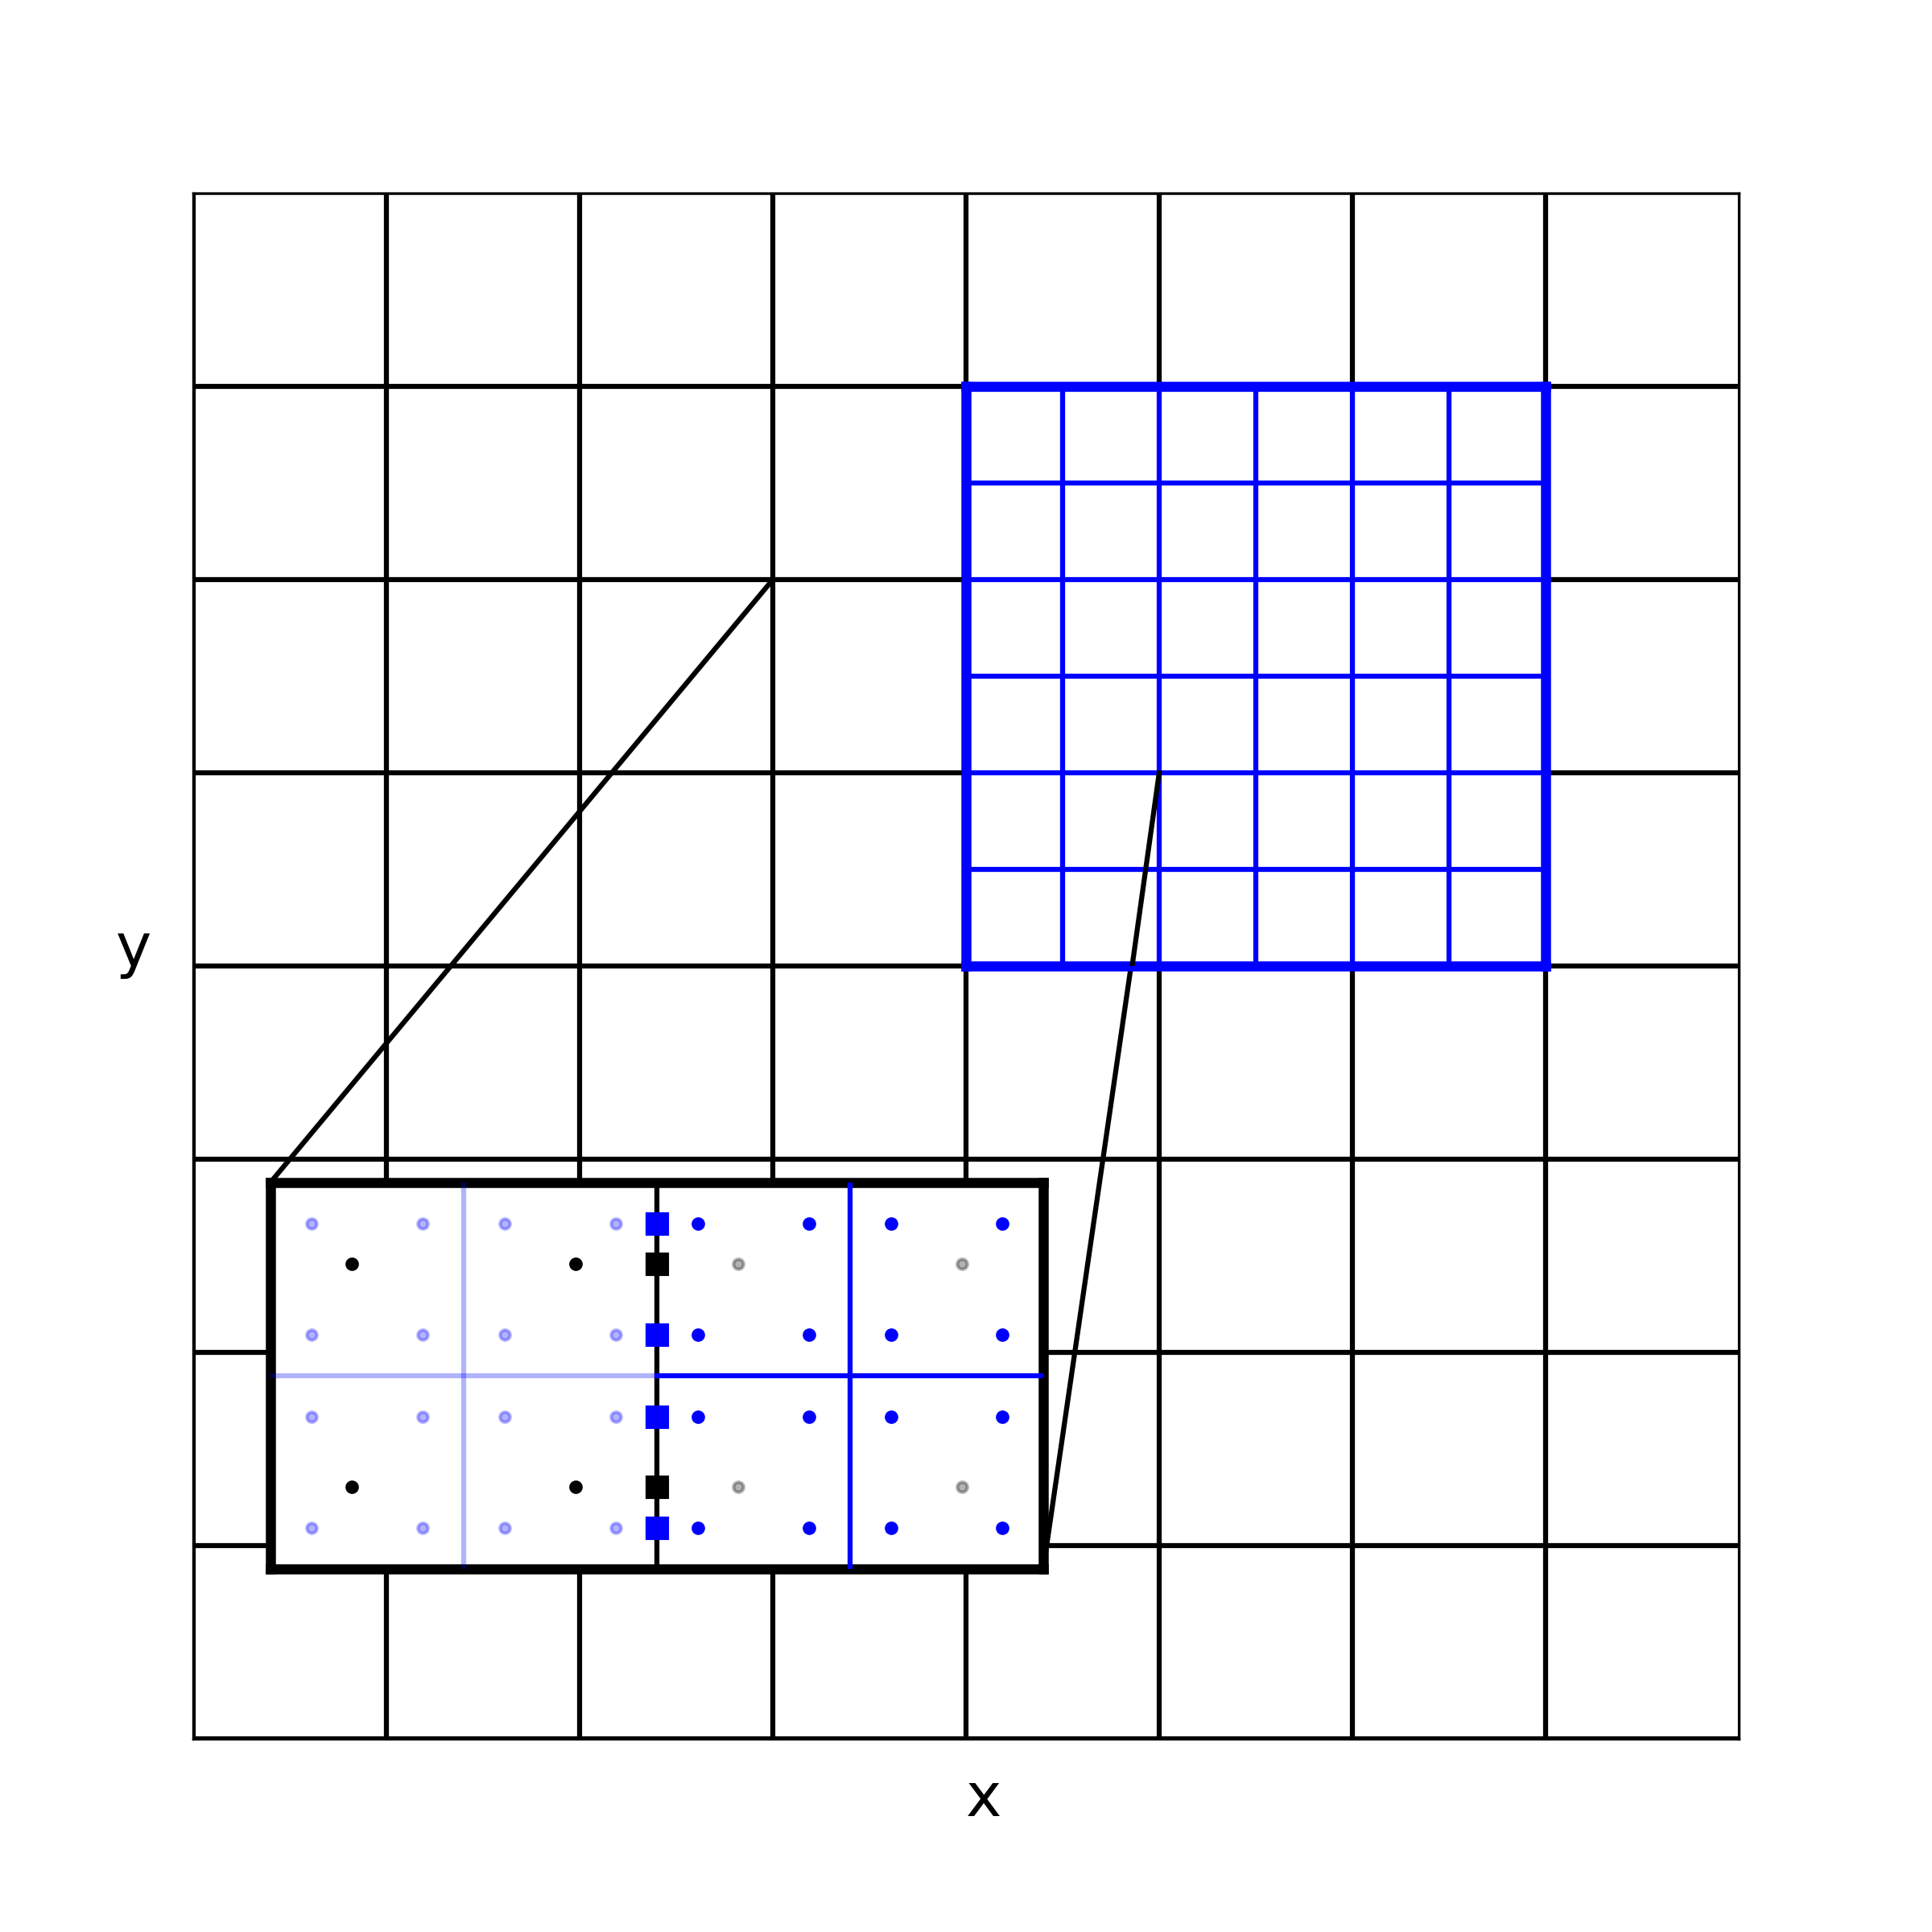
\includegraphics[width=0.5\textwidth]{fig.MeshRefinement_2D.png}
  \caption{Cartoon depicting a 2D mesh with two levels of refinement
  for a second-order DG method.
  The black lines mark the mesh element interfaces on the coarser level
  and the blue lines mark those on the finer level.
  The black dots denote the Legendre--Gauss quadrature points on the coarser
  level and the blue dots denote those on the finer level.
  The solid black squares denote the Legendre--Gauss quadrature points
  on the interface between two elements on the coarser level and the solid blue
  squares denote those between two elements on the finer level.
  The dots and lines with a degree of transparency should be viewed as
  belonging to ghost cells.
  }
  \label{fig.MR2D}
\end{figure}

%------------------------------------------------------------------------------%
\section{Results}

\subsection{Scaling Studies}

In addition to offering tools for mesh refinement, coupling to \amrex\
allows \thornado\ to run in parallel with MPI.
Because CCSN simulations are very computationally expensive,
any code aiming to simulate them must efficiently use all available
resources.
We present our results for both strong and weak scaling below.
All scaling results are shown for a "Bergamo" node on the ISAAC-NG
cluster at the University of Tennessee, Knoxville.

\subsubsection{Strong-Scaling}

Strong-scaling allows a code to solve a problem with a fixed size quicker when
more processes are used.
To examine the strong-scaling capability of \thornado, we run
a problem having 256x512=131,072 elements with
1, 2, 4, 8, 16, 32, 64, and 128 MPI processes.
Our results are shown in \figref{fig.SS}.
We see ideal scaling out to $\sim\mc{O}\left(10^{6}\right)$ degrees of freedom
per process, and then good, but less than ideal scaling after that.
(This is likely due to the cost of communication between MPI processes
dominating over the cost of computation on a patch of data.)
We use this number to inform our weak-scaling study, which is described next.
\begin{figure}[htb!]
  \centering
  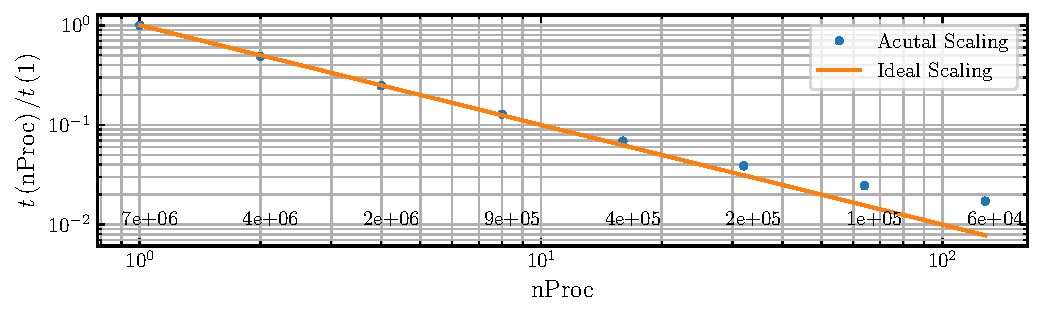
\includegraphics[width=0.8\textwidth]{fig.StrongScaling.pdf}
  \caption{The walltime to complete a simulation with nProc
processes, normalized to the walltime to complete the same simulation with one
process, plotted as a function of nProc.
Our data are shown as blue dots and the ideal scaling rate is shown as an
orange line.
The numbers reflect the approximate number of degrees of freedom per MPI
process for each simulation.}
  \label{fig.SS}
\end{figure}

\subsubsection{Weak-Scaling}

Weak-scaling allows a code to run larger problems that would otherwise
overwhelm the memory of a single processor.
To examine the weak-scaling capability of \thornado, we keep the number
of degrees of freedom per process fixed and increase the problem
size.
Given that we see ideal strong-scaling out to $\mc{O}\left(10^{6}\right)$
degrees of freedom per MPI process, we use that value for our single-process
weak-scaling reference.
Our results are shown in \figref{fig.WS}.
We see reasonable weak-scaling out to 32 MPI processes.
\ee{Were these results all obtained on the same hardware?
More details on the hardware should be given for all scaling results.}
\sd{I'm going to re-do both scaling studies on Summit
because I'll be able to use a lot more cores}
\begin{figure}[htb!]
  \centering
  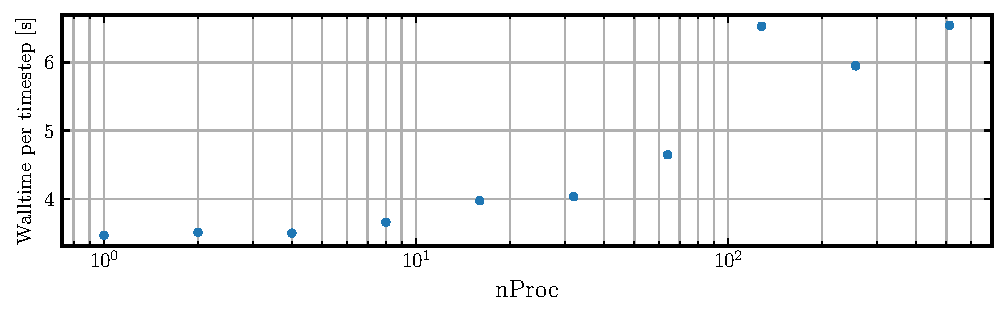
\includegraphics[width=0.8\textwidth]{fig.WeakScaling.pdf}
  \caption{The walltime per timestep versus the number of MPI processes.}
  \label{fig.WS}
\end{figure}

\subsection{Effects of Flux Corrections on Accuracy}

Our first test problem examines the effects of the flux corrections on the
accuracy of our numerical method.
We investigate this with the one-dimensional linear advection of a
smooth density profile using an ideal \eos\ with $\Gamma=4/3$
and periodic boundary conditions.
At $t=0$ the density, velocity, and pressure are set to
\begin{equation}
  \rho\left(x\right)=1+0.1\,\sin\left(2\pi x/L\right),
  \hspace{1em}v\left(x\right)=0.1,\hspace{1em}p\left(x\right)=1,
\end{equation}
with $x\in\left[0,L\right]$ and $t\in\left[0,L/v\right]$, with $L=1$.
For these simulations, we apply neither the slope limiter nor the
bound-enforcing limiter.
By allowing the profile to advect until it returns to its original state,
we can quantify the accuracy of our method via, e.g., the relative error of
the density, $E_{\rho}$, which we define as
\begin{equation}
  E_{\rho}
  :=\frac{\int_{\mc{D}}\left|\rho_{h}\left(L/v,x\right)
          -\rho_{h}\left(0,x\right)\right|\,dx}
         {\int_{\mc{D}}\left|\rho_{h}\left(0,x\right)\right|\,dx}.
  \label{eq.Error}
\end{equation}
In order to assess the effect of the flux corrections, we perform eight
simulations: four with a single-level mesh, two with a two-level mesh
where flux corrections are not applied,
and two with a two-level mesh where flux corrections are applied.
For the two-level mesh simulations, we place the (stationary)
refinement boundary at $L/2$.
Our results are shown in \tabref{tab.CR}.
% Generated by /home/kkadoogan/Work/Analysis/thornadoHydroXCFC_MethodsPaper_Software/./computeL1Error.py
% on 2024-02-03 17:43:15.562823
% Modified to work with Vanderbilt dissertation format
\begin{table}[b]
  \scriptsize
  \renewcommand{\tabcolsep}{0.09cm}
  \centering
  \begin{tabularx}{0.4\textwidth}{cccccc} \\
    \toprule \\
    $N$              &
    $\NK$            &
    Mesh             &
    Flux Corrections &
    $E_{\rho}$       \\ \\
    \midrule \\
2 & 32 & Single & N/A & $2.19\times10^{-5}$ \\
2 & 48 & Multi & Yes & $1.20\times10^{-5}$ \\
2 & 48 & Multi & No & $3.59\times10^{-4}$ \\
2 & 64 & Single & N/A & $5.13\times10^{-6}$ \\
3 & 32 & Single & N/A & $7.00\times10^{-6}$ \\
3 & 48 & Multi & Yes & $3.07\times10^{-6}$ \\
3 & 48 & Multi & No & $1.42\times10^{-5}$ \\
3 & 64 & Single & N/A & $9.77\times10^{-7}$ \\
  \bottomrule \\
  \end{tabularx}
  \caption{%
Effects of flux corrections on the accuracy
of our numerical method.
The first column is the number of DG nodes per element,
the second column is the number of elements,
the third column specifies whether or not the simulation used a single-
or multi-level mesh,
the fourth column specifies whether or not a multi-level mesh simulation
applied flux corrections,
and the fifth column denotes the error as defined in
\myeqref{eq.Error}.}
  \label{tab.CR}
\end{table}


The first point we note is that, for a given number of DG nodes and
a single-level mesh, the error decreases with increasing
resolution, as expected.
The second point we note that is that, defining $\NK$ as the number of
elements, when going from, e.g., $\NK=32$ with a single-level mesh
to $\NK=48$ with a two-level mesh and not applying flux corrections,
the error increases;
however, when going from $\NK=32$ with a single-level mesh
to $\NK=48$ with a two-level mesh and applying flux corrections,
the error decreases.
This demonstrates the importance of the flux corrections in this simple
scenario;
this effect is enhanced in more complicated flows.

\subsection{Sod's Shock Tube}

Our next test problem is the well-known (to those who know it well)
Sod shock tube \citep{s1978},
with open boundary conditions,
$\Gamma=4/3$,
$t\in\left[0,0.4\right]$,
$x\in\left[0,1\right]$ with the discontinuity situated at $x=0.5$,
and the left and right states of the fluid at $t=0$ given by
\begin{alignat*}{3}
  &\rho_{\textsc{l}}=1,\hspace{1em}
  &v_{\textsc{l}}=0,\hspace{1em}
  &p_{\textsc{l}}=1 \\
  &\rho_{\textsc{r}}=0.125,\hspace{1em}
  &v_{\textsc{r}}=0,\hspace{1em}
  &p_{\textsc{r}}=0.1.
\end{alignat*}
We refine the mesh based on the gradient of the density in order to capture
the shock and the contact discontinuity.
We obtain the exact solution for this problem with the code presented
in \citet{mm2003}.
Our results are shown in \figref{fig.Sod}.
The single-level mesh simulation ($\NK=256$) captures all discontinuities well.
The AMR simulation, which has $\NK=16$ on its coarsest level and $\NK=256$
on its finest level, captures the discontinuities as well as the single-level
mesh simulation and uses less degrees of freedom in the smooth regions; e.g.,
outside of the Riemann fan and in the post-shock and post-contact flow regions.
\begin{figure}[htb!]
  \centering
  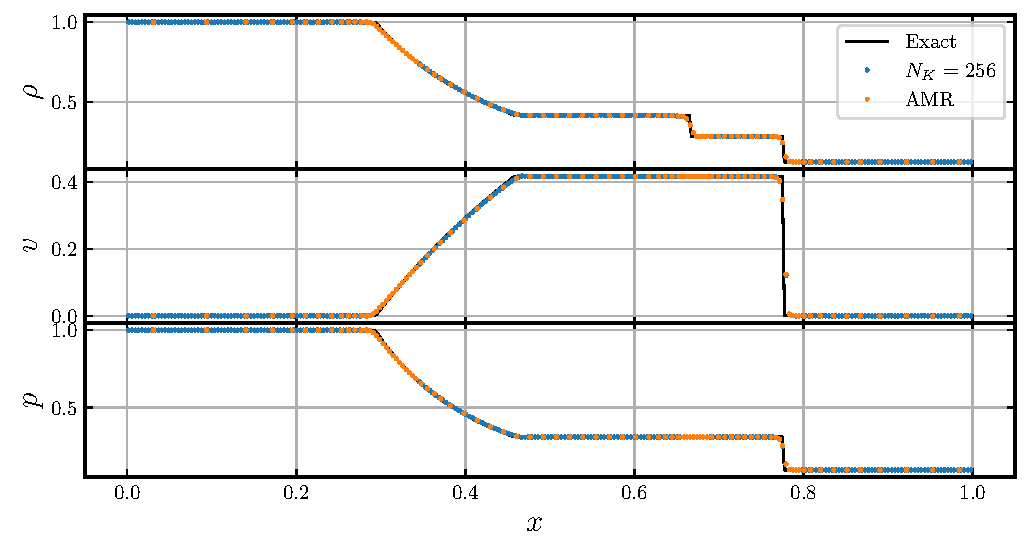
\includegraphics[width=0.9\textwidth]{fig.Sod.pdf}
  \caption{
Comoving baryon mass density (top-panel),
velocity (middle-panel),
and pressure (bottom-panel),
plotted as functions of $x$ at $t=0.4$ for the Sod shock tube problem.
Numerical results are shown as dots and
analytical results are shown as solid lines.
Single-level mesh results with $\NK=256$ are shown in blue
and five-level mesh results are shown in orange.}
  \label{fig.Sod}
\end{figure}

\subsection{2D Blast Wave}

Our next test is a 2D blast wave from \citet{db2002},
which tests the code's
ability to resolve strong shocks in multiple dimensions.
The setup for the problem is
$\Gamma=5/3$,
$t\in\left[0,0.4\right]$,
$x\times y\in\left[0,1\right]\times\left[0,1\right]$
with discontinuities located at $x=0.5$ and $y=0.5$,
open boundary conditions,
and the state of the fluid at $t=0$ given by
\begin{align}
\begin{split}
  \left(\rho_{\textsc{ne}},v^{1}_{\textsc{ne}},
  v^{2}_{\textsc{ne}},p_{\textsc{ne}}\right)
  &=\left(0.1,0,0,0.01\right) \\
  \left(\rho_{\textsc{nw}},v^{1}_{\textsc{nw}},
  v^{2}_{\textsc{nw}},p_{\textsc{nw}}\right)
  &=\left(0.1,0.99,0,1\right) \\
  \left(\rho_{\textsc{sw}},v^{1}_{\textsc{sw}},
  v^{2}_{\textsc{sw}},p_{\textsc{sw}}\right)
  &=\left(0.5,0,0,1\right) \\
  \left(\rho_{\textsc{se}},v^{1}_{\textsc{se}},
  v^{2}_{\textsc{se}},p_{\textsc{se}}\right)
  &=\left(0.1,0,0.99,1\right)
\end{split},
\end{align}
where the subscripts refer to the four quadrants of the domain
(north-east, north-west, south-west, south-east).
We perform two simulations: one using a single-level mesh and $256^{2}$
elements and another using a four-level mesh with $32^{2}$
elements on the coarsest level
and, therefore, $256^{2}$ elements on the finest level.
Both simulations have $N=3$ and $\NSSPRK=3$.
For the four-level mesh run, the tagging criteria are based
on the gradient of the density.
Our results are shown in \figref{fig.dZB2002}.
In the single-level mesh results (left panel),
the bow shock is well resolved.
The four-level mesh simulation (middle panel)
captures the shock with high resolution but, as can be seen in the right panel,
in regions outside the shock, the mesh is coarser, leading to a savings in
computation, walltime, and the size of the plotfiles.
Specifically, at the snapshot shown, the four-level mesh simulation has
21,736 leaf elements, while the single-level mesh simulation as 65,536
leaf elements.
There are features near
$x=0.6$, $y=0.6$, $x=0.2$, and $y=0.2$ that are clearly
visible in the single-level
mesh simulation, but are much fainter in the four-level mesh simulation.
This could likely be improved with an improved tagging criteria.
The same is true of the features near $x=0.85$ and $y=0.85$,
which are more diffusive in the four-level simulation
than they are in that of the single-level mesh.
\begin{figure}[htb!]
  \includegraphics[width=0.3\textwidth]%
    {fig.dZB2002_256x256.pdf}\hfill%
  \includegraphics[width=0.3\textwidth]%
    {fig.dZB2002_032x032_AMR.pdf}\hfill%
  \includegraphics[width=0.3\textwidth]%
    {fig.dZB2002_032x032_AMR_Mesh.pdf}
  \caption{Plots of the 2D blast wave from \citet{db2002}.
The left panel shows the pressure from
a single-level mesh simulation with $128^{2}$ elements,
the middle panel shows the pressure from a four-level mesh
simulation with $32^{2}$ elements on the coarsest level,
and the right panel shows the density from the same four-level
mesh simulation, and also overplots the mesh.}
  \label{fig.dZB2002}
\end{figure}

\subsection{3D Kelvin--Helmholtz}
\begin{itemize}
  \item Pretty pictures
  \item Turbulent energy cascade
  \item Numerical dissipation scale
  \item GPU speed-up?
\end{itemize}

Our last test is a 3D Kelvin--Helmholtz instability problem,
which tests the code's ability to resolve turbulent regions.
Our setup follows \cite{rr2012}, with
periodic boundary conditions in all three dimensions,
$t\in\left[0,TBD\right]$, and
$x\times y\times z\in\left[-0.5,+0.5\right]
\times\left[-1,+1\right]\times\left[-0.5,+0.5\right]$.
The shear velocity of the fluid at $t=0$ is given by
\begin{equation}
  v^{x}\left(x,y\right)
  =\begin{cases}
     +\Vshear\tanh\left[\left(y-y_{0}\right)/a\right] & y>0 \\
     -\Vshear\tanh\left[\left(y+y_{0}\right)/a\right] & y\leq0
   \end{cases},
\end{equation}
with $\Vshear=0.5$, $y_{0}=0.5$, and $a=0.01$;
the density profile is given by
\begin{equation}
  \rho\left(y\right)
  =\begin{cases}
     \rho_{0}+\rho_{1}\tanh\left[\left(y-y_{0}\right)/a\right] & y>0 \\
     \rho_{0}-\rho_{1}\tanh\left[\left(y+y_{0}\right)/a\right] & y\leq0
   \end{cases},
\end{equation}
with $\rho_{0}=0.505$ and $\rho_{1}=0.495$;
the pressure everywhere is set to unity and $\Gamma=4/3$.
This steady-state is perturbed by imposing a velocity profile in the vertical
direction of the form
\begin{equation}
  v^{y}\left(x,y\right)
  =\begin{cases}
     +A_{0}\,\Vshear\sin\left(2\pi x\right)
     \exp\left[-\left(y-y_{0}\right)^{2}/\sigma^{2}\right] & y>0 \\
     -A_{0}\,\Vshear\sin\left(2\pi x\right)
     \exp\left[-\left(y+y_{0}\right)^{2}/\sigma^{2}\right] & y\leq0
   \end{cases},
\end{equation}
with $A_{0}=0.1$ and $\sigma=0.1$.
The velocity in the $z$-direction is a random number between
$-0.01$ and $+0.01$, taken from a uniform distribution.

%------------------------------------------------------------------------------%
\section{Applications}

\subsection{SASI with AMR}

Our first application is the evolution of a 2D, general relativistic
standing accretion shock instability \citep[SASI,][]{bmd2003}.
A detailed description of the problem and our setup is described in
\citet{dem2023} (in press).
The only modifications we make are to setup the grid with multiple levels
and to use AMR.

\subsection{1D Adiabatic Collapse}

Our second application is the 1D evolution of a 15 Solar mass progenitor
from \citet{wh2007} through collapse, bounce, and post-bounce phases with the
SFHo \eos, including self-gravity.
We first compare a single-level mesh simulation with resolution of 0.5 km
to a five-level mesh simulation with resolution on the finest level of 0.5 km.
Our refinement scheme is based on the density: at each new decade, starting
from $\rho=10^{9}\,\g\,\cm^{-3}$, a new level is added.

\subsubsection{Validation of AMR Implementation}

Our results from the collapse phase are shown in \figref{fig.Collapse_0.5km}.
We see that, overall, the two simulations agree.
There are slight differences as the system becomes
more compact; i.e., the five-level mesh simultation seems to be evolving
slightly quicker, as can be seen by the dashed lines moving slightly ahead
of the solid lines.
This may be an artifact of the two simulations not writing plotfiles at
exactly the same times.
\begin{figure}[htb!]
  \centering
  \includegraphics[width=0.8\textwidth]%
    {fig.AdiabaticCollapse_Collapse_dr0.50km.pdf}
  \caption{%
Mass density in $\g\,\cm^{-3}$ (top-left),
fluid velocity normalized to the speed of light (top-right),
conformal factor (top of bottom-left),
lapse function (bottom of bottom-left),
and temperature in $\K$ (bottom-right),
plotted as functions of radius in kilometers for a single-level mesh
simulation (solid) and for a five-level mesh simulation (dashed).
Each line corresponds to the central density reaching a new decade.}
  \label{fig.Collapse_0.5km}
\end{figure}

Next, we discuss the post-bounce phase, the results from which are shown in
\figref{fig.PostBounce_0.5km}.
We again see general agreement with the single-level and five-level mesh
simulations.
We note differences in the post-shock entropy per baryon,
in particular, the oscillations in the flow are larger in the five-level mesh
simulation than in the single-level mesh simulation.
We attribute this to the coarser mesh in that region.
A tagging criteria that also accounts for the bounce shock may mitigate
this issue.
\begin{figure}[htb!]
  \centering
  \includegraphics[width=0.8\textwidth]%
    {fig.AdiabaticCollapse_PostBounce_dr0.50km.pdf}
  \caption{%
Mass density in $\g\,\cm^{-3}$ (top-left),
temperature in $\K$ (top-right),
electron fraction (bottom-left),
and entropy, $S$, per baryon in units of $\kb$ (bottom-right),
plotted as functions of radius for the same simulations as are shown in
\figref{fig.Collapse_0.5km}.
The snapshots are chosen such that the shock radius, $\rsh$, is,
for each simulation,
$\rsh/\left(10^{3}\,\km\right)=\left(0.1,0.5,1,2,4,7\right)$.}
  \label{fig.PostBounce_0.5km}
\end{figure}

\subsection{Resolution Study}

\sd{Compare amr runs with different numbers of levels.
During collapse, look at central quantities versus central density
and post-bounce, look at central quantities versus $t-t_{\mathrm{b}}$}

%------------------------------------------------------------------------------%
\section{Conclusions}

%------------------------------------------------------------------------------%
\section{Data Availability}

The data underlying this paper will be shared on reasonable request to the
corresponding author.

%------------------------------------------------------------------------------%

\section{Software}

\href{https://amrex-codes.github.io/}{AMReX}
\citep{zab2019},
\href{https://matplotlib.org/}{Matplotlib}
\citep{h2007},
\href{http://www.numpy.org/}{NumPy}
\citep{hmw2020},
\href{https://yt-project.org/}{yt}
\citep{tso2011}

\appendix

%------------------------------------------------------------------------------%
\section{Vector Components}

A generic four-vector, $u$, can be expanded in any coordinate basis
(e.g., the 3+1 coordinate basis),
$\left\{\p/\p x^{\mu}\right\}$, as
\begin{equation}
  u=u_{\left(x\right)}^{\mu}\,\pd{}{x^{\mu}},
\end{equation}
where $\p/\p x^{\mu}$ is the $\mu$-th basis vector
and $u_{\left(x\right)}^{\mu}$ is the $\mu$-th component of $u$ in
that basis.
In general, these basis vectors are not orthonormal;
i.e., $g\left(\p/\p x^{\mu},\p/\p x^{\nu}\right)
=:g^{\left(x\right)}_{\mu\nu}\neq\eta_{\mu\nu}$,
where, here, $g$ is the $\left(0,2\right)$ metric tensor.
We can also expand $u$ in an orthonormal basis, $\left\{e_{\mu}\right\}$,
\begin{equation}
  u=u^{\mu}\,e_{\mu},
\end{equation}
where the $e_{\mu}$ are defined such that
$g\left(e_{\mu},e_{\nu}\right)=\eta_{\mu\nu}$.
If $e_{0}$ is a four-velocity then this basis can be associated
with an observer, and $\left\{e_{\mu}\right\}$ can properly
be called a frame of reference.
In particular, if $e_{0}\equiv n$ (see \secref{ss.3+1}) then this frame defines
an Eulerian observer, and $\left\{e_{\mu}\right\}$ is the frame of
reference of an Eulerian observer.

As an example of immediate relevance,
the four-velocity of the fluid as measured by an Eulerian observer
in the 3+1 basis (in which the 0-th component is zero) is
\begin{equation}
  v=v_{\left(x\right)}^{\mu}\,\pd{}{x^{\mu}}
  =v_{\left(x\right)}^{i}\,\pd{}{x^{i}}.
\end{equation}
The $v_{\left(x\right)}^{i}$
are what we initialize in our test problems and applications.
In spherical-polar coordinates, this vector takes the form
\begin{equation}
  v=v_{\left(x\right)}^{r}\,\pd{}{r}
  +v_{\left(x\right)}^{\theta}\,\pd{}{\theta}
  +v_{\left(x\right)}^{\varphi}\,\pd{}{\varphi}.
\end{equation}
This should be contrasted with the perhaps more familiar form,
\begin{equation}
  v=v^{i}\,e_{i}
  =v^{r}\,e_{r}+v^{\theta}\,e_{\theta}
  +v^{\varphi}\,e_{\varphi},
\end{equation}
where
\begin{equation}
  e_{i}:=\left|\left|\pd{}{x^{i}}\right|\right|^{-1}\,
  \pd{}{x^{i}}\hspace{1em}\left(\mathrm{no\ sum\ over\ }i\right),
\end{equation}
with
\begin{equation}
  \left|\left|\pd{}{x^{i}}\right|\right|
  :=\left|g\left(\pd{}{x^{i}},
  \pd{}{x^{i}}\right)\right|^{1/2}
  =\left|g^{\left(x\right)}_{ii}\right|^{1/2}=h^{\left(x\right)}_{i},
\end{equation}
and where $h^{\left(x\right)}_{i}$ is the $i$-th scale factor in the
coordinate system $\left\{\p/\p x^{\mu}\right\}$.
From this, we see that the components of $v$ in the 3+1 basis,
$v_{\left(x\right)}^{i}$,
are related to the components of $v$ in the basis of the Eulerian
observer, $v^{i}$, as
\begin{equation}
  v^{i}
  =h^{\left(x\right)}_{i}\,v_{\left(x\right)}^{i}
  \ \left(\mathrm{no\ sum\ over\ }i\right).
\end{equation}

Also, note that the $v_{\left(x\right)}^{i}$ are different from
the coordinate velocities,
which are instead defined as (dropping the $\left(x\right)$ subscript)
\begin{equation}
  \dot{x}^{i}:=\td{x^{i}}{t}
  =\td{\tau}{t}\,\td{x^{i}}{\tau}
  =\frac{u^{i}}{u^{0}}
  =\frac{W}{u^{0}}\left(v^{i}+n^{i}\right)
  =\alpha\left(v^{i}+n^{i}\right)
  =\alpha\,v^{i}-\beta^{i}.
\end{equation}

